\documentclass[11pt]{article}

\usepackage{graphicx} % Required for inserting images
\usepackage{xcolor}
\usepackage[normalem]{ulem}
\newcommand{\TODO}[1]{{\color{purple}\textbf{TODO:} #1}}

\usepackage{amssymb, amsfonts, amsmath, amsthm, mathtools}
\usepackage[margin=1in, footskip=1cm, headheight = 1.5cm]{geometry}
\makeatletter\def\blx@noerroretextools{}\makeatother % autonum loads etextools; demote biblatex's error to a warning
\usepackage[style=ext-authoryear-comp, sorting=none, sortcites=true, maxcitenames=2, uniquename=false,
            uniquelist=false, natbib=true, backend=biber]{biblatex}
\DeclareOuterCiteDelims{parencite}{\bibopenbracket}{\bibclosebracket}
\DeclareInnerCiteDelims{textcite}{\bibopenbracket}{\bibclosebracket}
\addbibresource{bibliography.bib}
\usepackage{booktabs}
\usepackage{algorithm}
\usepackage{algorithmic}
\usepackage[hypertexnames=false]{hyperref}
\usepackage{microtype,booktabs,enumitem,array,longtable}
% Floats: keep figures on text pages near their paragraphs, build float pages
% only when they are nearly full, and never let a figure drift past its section.
\usepackage[section]{placeins}
\renewcommand{\topfraction}{0.85}
\renewcommand{\bottomfraction}{0.6}
\renewcommand{\textfraction}{0.1}
\renewcommand{\floatpagefraction}{0.8}
\setcounter{topnumber}{3}
\setcounter{totalnumber}{4}
\hypersetup{
    colorlinks=true,
    linkcolor=blue,
    citecolor=cyan,
    pdftitle={Expected Inner Work of Inexact Proximal Point Methods},
    pdfpagemode=UseOutlines,
    }
\usepackage[nameinlink,capitalize]{cleveref}
\usepackage{autonum}
\makeatletter
\AtBeginDocument{\autonum@generatePatchedReferenceCSL{Cref}}
\makeatother
% --- autonum + subequations: number the whole block when the block's own label is referenced ---
\makeatletter
\newif\ifautonum@forceNumbers
\newif\ifautonum@subeq@rollback
\let\autonum@possiblyHideNumberOrig\autonum@possiblyHideNumber
\def\autonum@possiblyHideNumber{\ifautonum@forceNumbers\else\autonum@possiblyHideNumberOrig\fi}
\AtBeginDocument{%
  \CsLetCsLtxMacro{autonum@subequationsOld}{subequations}%
  \CsLetCsLtxMacro{autonum@endsubequationsOld}{endsubequations}%
  \renewenvironment{subequations}{\autonum@subequationsOld}{%
    \ifautonum@forceNumbers\else\ifnum\value{equation}=0 \autonum@subeq@rollbacktrue\fi\fi % nothing inside got a number
    \autonum@endsubequationsOld
    \ifautonum@subeq@rollback\addtocounter{equation}{-1}\fi % give the parent number back
  }%
  % A \label issued at the subequations level (right after \begin{subequations}) whose key is
  % referenced switches on numbering for every line of the block.
  \LetLtxMacro\autonum@subeq@origLabel\label
  \def\label{\@ifnextchar[\autonum@subeq@label@opt\autonum@subeq@label@noopt}%
}
\def\autonum@subeq@label@noopt#1{\autonum@subeq@check{#1}\autonum@subeq@origLabel{#1}}
\def\autonum@subeq@label@opt[#1]#2{\autonum@subeq@check{#2}\autonum@subeq@origLabel[#1]{#2}}
\def\autonum@subeq@check#1{\ifdefstring{\@currenvir}{subequations}{\ifcsedef{autonum@#1Referenced}{\autonum@forceNumberstrue}{}}{}}
\makeatother
% Shared macros and environments for every document in tex/.
% Seeded from the group's standard template; project-specific additions are
% collected at the end.

% Commands
\newcommand{\eg}{{\it e.g.}}
\newcommand{\ie}{{\it i.e.}}

% Sets
\newcommand{\ones}{\mathbf 1}
\newcommand{\reals}{{\mathbf R}}
\newcommand{\integers}{{\mathbf  Z}}
\newcommand{\symm}{{\mathbf S}}  % symmetric matrices
\newcommand{\NPhard}{\mbox{$\mathcal{NP}$-hard}}
\newcommand{\prob}{{\mathbf P}}
\newcommand{\distrib}{{\mathcal P}}
\newcommand{\identity}{I}
\newcommand{\nullspace}{{\mathcal N}}
\newcommand{\range}{{\mathcal R}}
\newcommand{\Rank}{\mathop{\bf rank}}
\newcommand{\Tr}{\mathop{\bf Tr}}
\newcommand{\diag}{\mathop{\bf diag}}
\newcommand{\lambdamax}{{\lambda_{\rm max}}}
\newcommand{\lambdamin}{\lambda_{\rm min}}
\newcommand{\Expect}{{\bf E{}}}
\newcommand{\Co}{{\mathop {\bf Co}}} % convex hull
\newcommand{\dist}{\mathop{\bf dist{}}}
\newcommand{\argmin}{\mathop{\rm argmin}}
\newcommand{\argmax}{\mathop{\rm argmax}}
\newcommand{\epi}{\mathop{\bf epi}} % epigraph
\newcommand{\Vol}{\mathop{\bf vol}}
\newcommand{\dom}{\mathop{\bf dom}} % domain
\newcommand{\intr}{\mathop{\bf int}}

\newcommand{\sign}{\mathop{\bf sign}}
\newcommand{\round}{\mathop{\bf round}}

% Sections (for citation)
\newcommand{\Sec}{Section\;}

% Create theorems and other environments
\newtheorem{theorem}{Theorem}[section]  % Restart counter every section
\newtheorem{lemma}{Lemma}[section]  % Restart counter every section
\newtheorem{corollary}{Corollary}[theorem]  % Restart counter every theorem
\newtheorem{proposition}{Proposition}[section]
\newtheorem{assumption}{Assumption}[section]

\theoremstyle{definition}
\newtheorem{definition}{Definition}[section]
\newtheorem{problem}{Problem}[section]

\theoremstyle{remark}
\newtheorem{example}{Example}[section]
\newtheorem{exercise}{Exercise}[section]
\newtheorem{remark}{Remark}[section]

% Acronyms.  Defined only when the preamble loaded the glossaries package, so
% that this file can be \input from a document that does not use acronyms.
\makeatletter
\@ifundefined{newacronym}{}{%
  \newacronym{LP}{LP}{linear program}
  \newacronym{QP}{QP}{quadratic program}
  \newacronym{MIQP}{MIQP}{mixed-integer quadratic program}
  \newacronym{MIP}{MIP}{mixed-integer program}
  \newacronym{MILP}{MILP}{mixed-integer linear program}
  \newacronym{MINLP}{MINLP}{mixed-integer nonlinear program}
  \newacronym{sBB}{sBB}{spatial branch and bound}
  \newacronym{PWA}{PWA}{piecewise affine}
  \newacronym{SVM}{SVM}{support vector machines}
  \newacronym{ReLU}{ReLU}{rectified linear unit}
  \newacronym{CPU}{CPU}{central processing unit}
  \newacronym{GPU}{GPU}{graphics processing unit}
  \newacronym{MPC}{MPC}{model predictive control}
  \newacronym{ADMM}{ADMM}{alternating direction method of multipliers}
  \newacronym{ADP}{ADP}{approximate dynamic programming}
  \newacronym{FPGA}{FPGA}{field-programmable gate array}
  \newacronym{DRS}{DRS}{Douglas--Rachford splitting}
  \newacronym{RandNLA}{RandNLA}{randomized numerical linear algebra}
  \newacronym{CG}{CG}{conjugate gradients}
  \newacronym{GMRES}{GMRES}{generalized minimal residual method}
}
\makeatother

% Project-specific definitions
\newcommand{\prox}{\mathrm{prox}}
\newcommand{\R}{\mathbb{R}}
\newcommand{\Prob}{\mathbb{P}}

% Positive part of the logarithm, used in the inner-work bounds.
\newcommand{\logp}{\log_{+}}

% Zero set, graph, and fixed point set of an operator, in the style of \dom.
\newcommand{\zer}{\mathop{\bf zer}}
\newcommand{\gra}{\mathop{\bf gra}}
\newcommand{\fix}{\mathop{\bf fix}}


\newcommand{\Acal}{\mathcal{A}}
\newcommand{\Bcal}{\mathcal{B}}
\newcommand{\Ccal}{\mathcal{C}}
\newcommand{\Fcal}{\mathcal{F}}
\newcommand{\Dcal}{\mathcal{D}}
\newcommand{\Hcal}{\mathcal{H}}
\DeclarePairedDelimiter{\norm}{\lVert}{\rVert}

\DeclarePairedDelimiterX{\ip}[2]{\langle}{\rangle}{#1,#2}

% lowercase names
\crefname{equation}{}{}
\crefname{assumption}{assumption}{assumptions}
\crefname{algocf}{Algorithm}{Algorithms}


\title{Expected Inner Work of Inexact Proximal Point Methods}
\author{Pranav Reddy}
\date{\small \today \vspace{-5mm}}

\begin{document}
\maketitle
\begin{abstract}
    We consider a monotone inclusion problem in a Hilbert space.
    Under mild assumptions, it is known that the proximal point method converges to a zero of the operator, even with inexact computations of the resolvent.
    We extend this analysis to get an explicit $O(1/k)$ nonasymptotic convergence rate of the squared fixed point residual and an asymptotic $o(1/k)$ convergence rate, as well as a linear convergence rate in the presence of an error bound.
    Assuming access to a linearly convergent iterative procedure to compute the resolvent, we show that the method requires $O(\varepsilon^{-2})$ inner steps to find a point with $\dist(0,\mathcal{A}u) \leq\varepsilon$ for a general monotone inclusion problem.
    We validate our theoretical findings on numerical experiments and show that many popular algorithms are special cases of our framework and benefit from inexact computations.
\end{abstract}
\section{Introduction}
In this paper we consider the problem of a maximal monotone inclusion on a real Hilbert space $\Hcal$:
\begin{align}
    \text{find } x \text{ such that } 0 \in\Acal x, \label{eq:monotone-inclusion}
\end{align}
where $\Acal:\Hcal\rightrightarrows\Hcal$ is a maximal monotone operator.
A popular method for solving this problem is the proximal point method (PPM): for a stepsize $\gamma$, we try to solve the backward inclusion $x_k \in (I + \gamma\mathcal{A})x_{k+1}$.
PPM has a long history, going back to the original work of \citet{Martinet1970RegularisationDV}, but it is better known in the English-speaking world through Rockafellar's pioneering work on the subject \citep{rockafellar-ppm-paper,rockafellar1976monotoneoperatorsandppm}.
The operator $(I + \gamma\mathcal{A})^{-1}$ is known as the \emph{resolvent} of $\mathcal{A}$.
By Minty's theorem, it is single-valued and defined everywhere whenever $\Acal$ is maximal monotone \citep[Theorem 21.1]{bauschkeConvexAnalysisMonotone2017}. 
It is known that PPM includes general classes of operator splitting methods, such as Douglas--Rachford, Chambolle--Pock, and Davis--Yin splitting \citep{EcksteinBertsekasDouglasRachfordSplitting,chambollePockFirstOrderPrimalDualAlgorithm2011,davisThreeOperatorSplittingScheme2017}.
The intuition is that by regularizing via $\gamma$ and solving the inclusion problem, a previously difficult problem may be decomposed into a sequence of simpler operations that are easier to implement.
This broad idea finds many applications in convex optimization, with notable success stories such as the iterative shrinkage-thresholding algorithm (ISTA), its accelerated variant (FISTA), and the primal-dual hybrid gradient method for linear programming (PDLP) and its variants \citep{ISTA-original-paper,FISTA-original-paper,applegate2022practicallargescalelinearprogramming-pdlp-paper}.
For an introduction to the theory of monotone operators and their application in optimization, see \citet{Ryu_Yin_OptimizationMonotoneOperators}.

It is a curious and important fact in algorithm design that the resolvent computation need not be done exactly.
\citet{rockafellar-ppm-paper} first showed that it suffices to compute a sequence of iterates whose errors form a summable sequence.
\citet{EcksteinBertsekasDouglasRachfordSplitting} extended the result to show that Douglas--Rachford is an instance of PPM and therefore it suffices to compute iterates whose approximation errors are summable.
This type of criterion is known as an \emph{absolute} error condition, since it controls the absolute error between the estimated update and the true resolvent.
However, there are several practical issues with such a condition.
First, checking the error condition requires knowledge of the true update, which is generally not computable.
Second, the choice of such a sequence adds an infinite number of parameters for the user to tune, making practical implementations difficult.
Moreover, the theory does not provide meaningful guidance on the design of such a sequence, nor does it provide guidance on how the degree of error affects the convergence of the algorithm and the complexity of intermediate computation.

To obviate this difficulty, we would like the error condition to have two properties.
First, it should be easy to compute, and not require knowledge of the true update.
Second, it should not depend on an external sequence of errors, but rather be a function of the current state of the algorithm in some way: a \emph{relative} error condition.
% To obviate this difficulty, it would be nice to have a \emph{relative} error criterion: one where the tolerance is a function of the current state of the algorithm (e.g., the fixed point residual of the iterates).
% This would provide meaningful guidance on the difficulty of solving a particular subproblem, as well as making tuning the algorithm parameters significantly easier.
\citet{EcksteinRelativeError2018} provide an affirmative answer to the question of designing a relative error criterion for Douglas--Rachford and the alternating direction method of multipliers (ADMM), and their result was extended by \citet{svaiter2018weaklyconvergentfullyinexact,BarrePEPInexactMethods}.

More recently, \citet{bredies2021degeneratepreconditionedproximalpoint} showed that many existing operator splitting methods, such as Chambolle--Pock, Douglas--Rachford, Peaceman--Rachford, and Davis--Yin, are instances of \emph{degenerate preconditioned} proximal point methods.
That is, we precondition the monotone inclusion problem \Cref{eq:monotone-inclusion} by replacing the scalar stepsize $\gamma$ with a matrix $\mathcal{M}\succeq 0$ and evaluating $(I + \mathcal{M}^{-1}\Acal)^{-1} = (\mathcal{M} + \Acal)^{-1}\mathcal{M}$.
Under mild assumptions, even when $\mathcal{M}$ is not invertible, the operator $(\mathcal{M} + \Acal)^{-1}\mathcal{M}$ still exists and can be computed.
These ideas can be generalized to relatively inexact resolvent evaluations with a broader class of preconditioners, such as in \citet{alves2025generalframeworkinexactsplitting}.

However, an analysis of the \emph{inner} complexity, the complexity of computing $x_{k+1}\approx (I + \mathcal{M}^{-1}\Acal)^{-1}x_k$, and its relationship to the convergence of PPM is more delicate. %has been missing in the literature.
\citet{machart2012optimalcomputationaltradeoffinexact} consider the complexity of inexact proximal gradient methods, but they only consider the case of absolute errors, with the standard summability conditions.
Moreover, they only consider a specific instance of an algorithm, whereas our setting is general enough to cover many more operator splitting methods.
\citet{LinMairal2018CatalystAcceleration} consider a model of global complexity, factoring in inner and outer complexity, but their error criterion is not generally computable, requiring knowledge of the exact solution to the subproblem or access to the dual function.
\citet{alves2017iterationcomplexityinexactdouglasrachford} provide analysis in a similar setting but only show asymptotic guarantees of inner complexity.

Our contributions are as follows:
\begin{enumerate}
    \item We modify \citet[Algorithm 1]{alves2025generalframeworkinexactsplitting} to analyze a practical stopping criterion and provide bounds on the error at stopping (\Cref{prop:certificate}).
    \item We improve the analysis of \citet{alves2025generalframeworkinexactsplitting} to get an explicit convergence rate as well as linear convergence in the presence of an error bound (\Cref{thm:convergence-guarantee,thm:error-bound-outer-convergence-guarantee}).
    \item We analyze the total inner work done over the course of the algorithm and show that the method requires $O(\varepsilon^{-2})$ inner steps to find a point with $\dist(0,\mathcal{A}u) \leq\varepsilon$ for a general monotone inclusion problem (\Cref{thm:total-inner-work-bound}).
    \item We analyze our results on some model choices of algorithms, such as PPM and ADMM, and infer some principled guidelines on selecting algorithm parameters (\Cref{prop:optimal-sigma-gradient-descent-inside-ppm,prop:admm}).
    \item We compare our theoretical results against empirical studies and find that the theorems are often conservative.
    In fact, most instances benefited from decreased accuracy (\Cref{sec:numerical-experiments}).
\end{enumerate}

\subsection{Setting and Notation}
We assume we have access to a linear map $\Ccal:\Dcal\to\Hcal$ between Hilbert spaces $\Dcal$ and $\Hcal$, which we refer to as a \emph{degenerate preconditioner}.
More precisely, the preconditioner is $\mathcal{M} = \Ccal\Ccal^*$, but through an abuse of terminology we will conflate the two objects.
For an operator $\mathcal{S}$, we define the zero set $\zer \mathcal{S} := \{u \mid 0 \in \mathcal{S} u\}$, the fixed point set $\fix\mathcal{S} := \left\{ u \mid u\in\mathcal{S}u \right\}$, and the graph $\gra \mathcal{S} := \left\{ (u,z) \mid z \in \mathcal{S}u \right\}$.
We define the resolvent of an operator $\mathcal{S}$ as $J_{\mathcal{S}} := (I + \gamma\mathcal{S})^{-1}$, and its fixed point residual operator as $R_{\mathcal{S}} := I - J_{\mathcal{S}}$.
Note that $\fix J_{\mathcal{S}} = \zer R_{\mathcal{S}} = \zer\mathcal{S}$.
In general, we will not use $R$ or $J$ to refer to operators other than $\Bcal$ defined in \Cref{def:b-definition}, so we drop the subscript and use the standing assumption that the underlying operator referred to is $\Bcal$.

An unspecified norm $\norm{x}$ refers to either the standard Euclidean norm or the induced norm of the ambient Hilbert space $\Hcal$.
Which norm is being referred to will be clear from context.
We denote the adjoint operator with a $*$, i.e., $\ip{\Ccal u}{v} = \ip{u}{\Ccal^* v}$.
For Euclidean space, this coincides with the transpose of a matrix, which we denote with $\top$.
We use $\log_+ := \max\{0,\log\}$ to denote the positive part of the logarithm.

The variables $u$, $w$, $y$, and $z$ are always used in a way that matches their use in \Cref{alg:stopping-time-algorithm}.
The reader should always assume that we are trying to find $u$, $w$, $y$, and $z$, such that $\Ccal z \in \Acal u$, $\gamma z + \Ccal^* u \approx w$, and $y = \Ccal^* u$.
The symbol $\gamma$ is always used to refer to the proximal parameter, also referred to as the stepsize.
Similarly, $\sigma$ will always be used to refer to the inexactness parameter of \Cref{alg:stopping-time-algorithm}, and $s$ is the stride, the number of inner iterations between inexactness checks.
We follow the convention that superscript indices refer to inner iterations and subscript indices refer to outer iterations

For convenience, we include a table outlining commonly used symbols and their meaning.
{\small
\renewcommand{\arraystretch}{1.14}
\begin{longtable}{@{}>{\raggedright\arraybackslash}p{0.23\textwidth}
                        >{\raggedright\arraybackslash}p{0.73\textwidth}@{}}
\toprule
Symbol & Meaning \\
\midrule
\endfirsthead
\toprule
Symbol & Meaning (continued) \\
\midrule
\endhead
\bottomrule
\endfoot
$\Acal$, $\Ccal$ & Original monotone operator $\Acal:\Hcal\rightrightarrows\Hcal$ and preconditioner factor $\Ccal:\Dcal\to\Hcal$. The original preconditioner is $\Ccal\Ccal^*$. \\
$\Bcal$ & The monotone operator used to write \Cref{alg:stopping-time-algorithm} as a proximal point method. \\
$J$, $R$ & The resolvent $J = (I+\gamma \Bcal)^{-1}$ and its fixed point residual $R = I - J$. \\
$s$ & The stride: the integer number of inner iterations between inexactness checks. \\
$\sigma$ & Inexactness tolerance parameter. \\
$\gamma$ & Stepsize or proximal parameter. \\
$\delta$ & Stopping tolerance. \\
$\alpha$ & Contraction parameter of the inner solver. \\
$C_0$ & Initialization constant of the inner solver. \\
$G_\sigma$, $H_\sigma$ & The warm-start constants of \Cref{lem:warm-start-bounds}. \\
$D$ & Constant factor relating to inexactness, $D := \frac{(1+\sigma)^2C_0G_\sigma^2}{\sigma^2}$. \\
$u$, $w$, $y$, $z$ & Iterates of the proximal point method with $\Ccal z \in \Acal u$, $\gamma z + \Ccal^* u \approx w$, and $y = \Ccal^* u$. Sometimes written with super- or subscripts to specify inner or outer iterations. \\
$K_\delta$ & Stopping time of the algorithm. The outer iteration at which $\norm{z_{k}} \leq \delta$. Equivalently, the number of accepted updates before stopping. \\
$K_\delta^+$ & Upper bound on the above. \\
$\prob_k$, $\Expect_k$ & The conditional probability and expectation at the start of outer iteration $k$, given all randomness generated before the $k$th inner solve begins. \\
$N_k$ & Number of inner iterations performed during outer iteration $k$. \\
\end{longtable}
}

We make the following assumption to ensure that all the operations we take in this paper are well-defined.
\begin{assumption}\label{assumption:well-defined-resolvents}
    We assume that $\Acal$ is a maximal monotone operator $\Acal: \Hcal \rightrightarrows \Hcal$ on the Hilbert space $\Hcal$ with at least one zero: $\zer \Acal \neq\varnothing$.
    We assume that the map $\Ccal:\Dcal\to\Hcal$ is a bounded linear map between Hilbert spaces, that $\Ccal^*$ is surjective, and that $(\Ccal\Ccal^* + \gamma\Acal)^{-1}\Ccal\Ccal^*$ is defined everywhere.
\end{assumption}

\begin{definition}\label{def:b-definition}
Define the operator $\Bcal$ by its graph as
\begin{equation}
    \gra{\Bcal} = \{ (\Ccal^* u, z) \mid \Ccal z\in\Acal u\}.
\end{equation}
\end{definition}
% For simplicity, assume that $\Acal u = \nabla f(u)$, where $f$ is a smooth convex function, and assume $\Ccal = I$ for simplicity.
% Then, the operator $\Bcal = \Acal = \nabla f$, and the analysis below reduces to that of the proximal point method on a smooth convex function.
% To connect this with the discussion above, suppose $\Ccal\Ccal^* = M \succ 0$ and $A$ is single-valued.
% Then, in item 2 of \Cref{lem:B-properties}, we can see that $Cu = Mv + \gamma Cz$
% To get more intuition behind the definitions, see \citet{alves2025generalframeworkinexactsplitting}.
Since $\Ccal^*$ is surjective (\Cref{assumption:well-defined-resolvents}), the resolvent $J := (I+\gamma \Bcal)^{-1}$ is defined on the entire space $\Dcal$ (\Cref{lem:B-properties}).
Note that $\Bcal$ itself need not have full domain.
In particular $\dom \Bcal \subseteq \Ccal^*\dom\Acal$, with strict inclusion a possibility.
One way of viewing this definition is that $\Bcal$ is a projection of $\Acal$ onto a lower-dimensional space.
\Cref{prop:admm} shows that this perspective enables us to view the iterates of ADMM as the projections of a higher-dimensional PPM.
\begin{lemma}\label{lem:B-properties}
    For $\Bcal$ defined as in \Cref{def:b-definition}, under \Cref{assumption:well-defined-resolvents}, the following hold:
    \begin{enumerate}
        \item $\zer{\Bcal} = \Ccal^* \zer{\Acal}$.
        \item For $x\in\Dcal$, $w = (I+\gamma \Bcal)^{-1}x$ if and only if there exist $v\in\Hcal$ and $z\in\Dcal$ such that $x = \Ccal^* v + \gamma z$, $\Ccal z \in \Acal v$, and $w = \Ccal^* v$. Moreover, such $v$ and $z$ exist for every $x\in\Dcal$.
        \item $\Bcal$ is maximal monotone.
    \end{enumerate}
\end{lemma}
\begin{proof}
        The first claim is immediate.
        The second follows from \Cref{assumption:well-defined-resolvents} and manipulating the definition of $\Bcal$:
\begin{align}
    (I+\gamma \Bcal)^{-1}x = w &\iff x \in (I+\gamma \Bcal)w \\
    &\iff x \in (I+\gamma \Bcal)w, \ w = \Ccal^* v \text{ for some } v \text{ with } \Ccal^*v \in \dom\Bcal \\
    &\iff x = \Ccal^* v + \gamma z, \ \Ccal z \in \Acal v, \ w = \Ccal^* v.
\end{align}
For existence, fix $x\in\Dcal$ and, since $\Ccal^*$ is surjective, we can write $x = \Ccal^*\tilde x$.
By \Cref{assumption:well-defined-resolvents} there exists $v$ with $\Ccal\Ccal^*\tilde x \in (\Ccal\Ccal^* + \gamma\Acal)v$, i.e., $\gamma^{-1}\Ccal\Ccal^*(\tilde x - v)\in\Acal v$.
Setting $z = \gamma^{-1}\Ccal^*(\tilde x - v)$ gives $\Ccal z\in\Acal v$ and $\Ccal^* v + \gamma z = \Ccal^*\tilde x = x$.

The third item follows from the fact that
\begin{align}
    \ip{\Ccal^* u_1 - \Ccal^* u_2}{z_1-z_2} = \ip{u_1 - u_2}{\Ccal z_1-\Ccal z_2} \geq 0,
\end{align}
since $\Ccal z_i\in\Acal u_i$ and $\Acal$ is monotone.
Maximality follows from \Cref{assumption:well-defined-resolvents}: by item 2, $\range(I+\gamma \Bcal) = \Dcal$, so $\Bcal$ is maximal by Minty's theorem \citep[Theorem 21.1]{bauschkeConvexAnalysisMonotone2017}.
\end{proof}

In the case where $\mathcal{A}$ is not necessarily monotone, it may still hold that $\Bcal$ is maximal monotone.
We make this assumption explicit.
\begin{assumption}\label{assumption:well-defined-b-operator}
    We assume that $\Bcal$ defined in \Cref{def:b-definition} is a maximal monotone operator.
    We also assume that the map $\Ccal:\Dcal\to\Hcal$ is a bounded linear map between Hilbert spaces with $\Ccal^*$ surjective.
\end{assumption}
Note that \Cref{assumption:well-defined-resolvents} is strictly stronger than \Cref{assumption:well-defined-b-operator}.
\Cref{prop:davis-yin} shows an example where \Cref{assumption:well-defined-b-operator} holds but \Cref{assumption:well-defined-resolvents} fails.

\section{The Degenerate Preconditioned Proximal Point Method}
The idea behind \citet[Theorem 1]{alves2025generalframeworkinexactsplitting} is that we would like to compute the resolvent $J := (I+\gamma \Bcal)^{-1}$, but this may be difficult.
Instead, we define a relative error criterion such that the computed iterates lie in the graph of $\Bcal$ and satisfy error bounds on how far from the true update they can be (\Cref{lem:exact-inexact-graph-pair-inequalities}).

To do this, we consider a modified version of the algorithm of \citet{alves2025generalframeworkinexactsplitting} (\Cref{alg:stopping-time-algorithm}), where we introduce a stopping rule for the inner loop.
The stopping rule is critical for the analysis of stopping times.
\Cref{prop:certificate} shows that the point returned by the terminal test is an approximate solution with an approximate optimality certificate, and \Cref{thm:convergence-guarantee} shows that the algorithm terminates after finitely many accepted updates.

\begin{algorithm}
\caption{Modified version of the algorithm from~\citet{alves2025generalframeworkinexactsplitting}.}\label{alg:stopping-time-algorithm}
\begin{algorithmic}[1]
\STATE \textbf{Initialize:} $w_0 \in \Dcal$, inexactness $\sigma \in [0,1)$, stepsize $\gamma > 0$, stride $s \in\mathbb{N}$, and stopping tolerance $\delta$
\FOR{$k = 0, 1, 2, \ldots$}
  \STATE Produce a pair $(u_{k}, z_{k}) \in \Hcal \times \Dcal$ with
  \[
    \Ccal z_{k} \in \Acal u_{k}, \qquad
    \gamma z_{k} + \Ccal^* u_{k} \approx w_k.
  \]
    \IF {$\norm{z_{k}} \leq \delta$}
        \STATE Stop and return $(z_{k}, u_{k}, w_{k})$.
    \ELSIF {$\norm{\gamma z_{k} + \Ccal^* u_{k} - w_k} \leq \sigma \norm{\Ccal^* u_{k} - w_k}$}
        \STATE Set $w_{k+1} = w_k - \gamma z_{k}$.
    \ELSE
        \STATE Improve the pair $(u_{k}, z_{k}) \in \Hcal \times \Dcal$ with $\Ccal z_{k} \in \Acal u_{k}$ via the iterative procedure $s$ times and go to line 4.
    \ENDIF
\ENDFOR
\end{algorithmic}
\end{algorithm}

The following proposition shows that at stopping, the returned iterates provide a certificate of distance to optimality.
Equivalents of the results in this section can be found in \citet{rockafellar1976monotoneoperatorsandppm,bredies2021degeneratepreconditionedproximalpoint,alves2025generalframeworkinexactsplitting} (among others), but we present modifications here for our purposes.
\begin{proposition}\label{prop:certificate}
    Every output from the $\norm{z}\leq\delta$ terminal test of \Cref{alg:stopping-time-algorithm} satisfies
    \begin{equation}\label{eq:original-certificate}
    \Ccal z\in\Acal u,\qquad
    \dist(0,\Acal u)\leq\norm{\Ccal z}
    \leq \norm{\Ccal}\delta.
    \end{equation}
    % Recall that the operator $\Bcal$ is defined by its graph as
    % \begin{equation}
    %     \gra{\Bcal} = \{ (\Ccal^* u, z) : \Ccal z\in\Acal u\}.
    % \end{equation}
    % and we also defined $J=(I+\gamma \Bcal)^{-1}$ and $R=I-J$ (see \Cref{def:b-definition}).
    Moreover, after stopping we also have
    \begin{equation}\label{eq:terminal-fp}
    \norm{ \Ccal^* u - J\Ccal^* u}\leq \gamma\delta.
    \end{equation}
    That is, the fixed point residual also satisfies the bound at halting.
    Note that the returned iterate may not satisfy the relative error criterion.
\end{proposition}
\begin{proof}
    The first claim is immediate from the definition of \Cref{alg:stopping-time-algorithm}.
    For the second, let $q=\Ccal^* u - J\Ccal^* u = (I-J)\Ccal^* u$.
    Then,
    \begin{equation}
        \left(\Ccal^* u -q,\frac{q}{\gamma}\right) = \left(J\Ccal^* u, \frac{q}{\gamma}\right) = \left(J\Ccal^* u,\frac{(I-J)\Ccal^* u}{\gamma}\right).
    \end{equation}
    Using \Cref{assumption:well-defined-b-operator}, there exists $x$ such that $\Ccal^* x = J \Ccal^*u$.
    Then,
    \begin{align}
        \Ccal^* x = (I+\gamma \Bcal)^{-1}\Ccal^* u &\iff  \Ccal^* u \in \Ccal^*x + \gamma \Bcal \Ccal^*x \\
        &\iff  \Ccal^* u = \Ccal^*x + \gamma \xi, \Ccal \xi \in \Acal x \\
        &\iff  \frac{\Ccal^* (u - x)}{\gamma} = \xi, \Ccal \xi \in \Acal x.
    \end{align}
    Thus, we can write 
    \begin{align}
        \left(J\Ccal^* u,\frac{(I-J)\Ccal^* u}{\gamma}\right) &= (\Ccal^* x, \gamma^{-1}\Ccal^* (u - x)) ,\quad \frac{\Ccal^* (u - x)}{\gamma} = \xi, \Ccal \xi \in \Acal x \\
        &= (\Ccal^* x, \xi) ,\quad \frac{\Ccal^* (u - x)}{\gamma} = \xi, \Ccal \xi \in \Acal x,
    \end{align}
    so $\left(\Ccal^* u -q,\frac{q}{\gamma}\right)\in\gra \Bcal$.
    Since $(\Ccal^* u, z) \in\gra \Bcal$ and $\Bcal$ is monotone,
    \begin{align}
        0 \leq \ip{(\Ccal^* u -q) - \Ccal^* u}{\frac{q}{\gamma} - z} = \ip{q}{z-\frac{q}{\gamma}}.
    \end{align}
    Thus, $\ip{q}{\gamma z-q}\geq0$ and hence
    \begin{align}
        \norm{\gamma z}^2 = \norm{\gamma z - q}^2 + 2\ip{\gamma z - q}{q} + \norm{q}^2 \geq \norm{q}^2.
    \end{align}
    Applying the stopping rule $\norm{z_k} \leq \delta$ from \Cref{alg:stopping-time-algorithm} (line 4) completes the proof.
\end{proof}

\section{Outer Convergence Guarantees}\label{sec:outer-convergence-guarantees}
In this section, we present a quantitative estimate on the convergence of \Cref{alg:stopping-time-algorithm}.
We will show that the inexactness affects convergence only through a multiplicative factor, which allows the rest of the analysis to follow.
The next lemma is needed to show the convergence of \Cref{alg:stopping-time-algorithm}.
\begin{lemma}\label{lem:exact-inexact-graph-pair-inequalities}
    The maps $J := (I+\gamma \Bcal)^{-1}$ and $R := I - J$ (the fixed point residual) are firmly nonexpansive.
    If $(y,z)\in\gra{\Bcal}$ is a candidate update pair (as in line 3 of \Cref{alg:stopping-time-algorithm} with $y = \Ccal^* u$) at $w$, then
    \begin{align}
        y &= J(\gamma z + y),\label{eq:resolvent-identity-y} \\
        \gamma z &= R(\gamma z + y), \label{eq:fixed-point-identity-z} \\
        \norm{y-J(w)}^2 + \norm{\gamma z-R(w)}^2 &\leq \norm{\gamma z + y - w}^2. \label{eq:graph-error-component-bound}
    \end{align}
    If the pair $(y,z)$ passes the relative test, then we also have
    \begin{align}
        (1-\sigma)\norm{y-w} \leq &\norm{R(w)} \leq (1+\sigma)\norm{y-w}, \label{eq:fixed-point-resolvent-bound} \\
        (1-\sigma)\norm{y-w} \leq &\norm{\gamma z} \leq (1+\sigma)\norm{y-w}, \label{eq:fixed-point-update-bound}\\
        \norm{\gamma z + y - w} &\leq \frac{\sigma}{1-\sigma}\norm{R(w)}, \label{eq:fixed-point-vs-error-bound}\\
        \norm{\gamma z} &\leq \frac{\norm{R(w)}}{1-\sigma}.\label{eq:fixed-point-update-vs-resolvent-bound}
    \end{align}
    Moreover, $\norm{R(w)} \leq \dist{(w,\zer \Bcal)}$.
\end{lemma}
\begin{proof}
    For the first equation, note that $y = \Ccal^*u$ and thus
    \begin{align}
        y &= J(\gamma z + y) \iff \gamma z + y \in y + \gamma \Bcal y \iff z \in \Bcal\Ccal^* u,
    \end{align}
    which is the definition of $\Bcal$.
    Next,
    \begin{align}
        R(\gamma z + y) = \gamma z + y - J(\gamma z + y) = \gamma z + y - y = \gamma z.
    \end{align}
    Firm nonexpansiveness follows from \Cref{assumption:well-defined-b-operator} and the firm nonexpansiveness of resolvents of maximal monotone operators \citep[Corollary 23.11]{bauschkeConvexAnalysisMonotone2017}.
    
    Next, by the monotonicity of $\Bcal$,
    \begin{align}
        \ip{y_1-y_2}{z_1-z_2} \geq 0,
    \end{align}
    so $\ip{y_1-y_2}{\gamma z_1-\gamma z_2} \geq 0$ as well.
    For an exact pair, $w = y+\gamma z$ with $z \in \Bcal y$,
    \begin{align}
        \norm{w_1-w_2}^2 &= \norm{\gamma z_1-\gamma z_2}^2 + \norm{y_1-y_2}^2 + 2\ip{y_1-y_2}{\gamma z_1-\gamma z_2} \\
        &\geq \norm{\gamma z_1-\gamma z_2}^2 + \norm{y_1-y_2}^2. \label{eq:component-bound-expansiveness}
    \end{align}
    Note that since $w = y+\gamma z$ with $z \in \Bcal y$, we have $y = J(w)$ and $\gamma z = R(w)$.
    That is, \Cref{eq:component-bound-expansiveness} states $\norm{w_1-w_2}^2 \geq \norm{R(w_1)-R(w_2)}^2 + \norm{J(w_1)-J(w_2)}^2$ for all $w_1$ and $w_2$.

    Let $e = \gamma z + y -w$, the graph residual.
    Note that $w + e = \gamma z + y$.
    Since $y = J(\gamma z + y) = J(w+e)$,
    \begin{equation}
        \gamma z = w + e - y = w + e - J(w+e) = (I-J)(w+e) = R(w+e).
    \end{equation}
    Thus, using the resolvent identities $y= J(\gamma z +y)$ and $\gamma z = R(\gamma z + y)$ \Cref{eq:resolvent-identity-y,eq:fixed-point-identity-z} and the component bound $\norm{w_1-w_2}^2 \geq \norm{\gamma z_1 - \gamma z_2}^2 + \norm{y_1 - y_2}^2$ \Cref{eq:component-bound-expansiveness} with $w_1 = w+e$ and $w_2 = w$,
    \begin{align}
        \norm{e}^2 = \norm{(w+e)-w}^2 &\geq \norm{R(w+e)-R(w)}^2 + \norm{J(w+e)-J(w)}^2 \\
        &= \norm{R(\gamma z + y)-R(w)}^2 + \norm{J(\gamma z + y)-J(w)}^2 \\
        &= \norm{\gamma z-R(w)}^2 + \norm{y-J(w)}^2.
    \end{align}

    Now suppose the relative test $\norm{e}\leq\sigma\norm{y-w}$ holds.
    By the reverse triangle inequality,
    \begin{align}
        |\norm{y-w} - \norm{R(w)}| = |\norm{y-w} - \norm{w - J(w)}| \leq \norm{y-J(w)} \leq \norm{e} \leq \sigma\norm{y-w}.
    \end{align}
    This is the residual bound \Cref{eq:fixed-point-resolvent-bound}.
    Next, $\gamma z = e - (y - w)$, so the triangle inequality gives
    \begin{align}
        (1-\sigma)\norm{y-w} \leq \norm{y-w} - \norm{e} \leq \norm{\gamma z} \leq \norm{y-w} + \norm{e} \leq (1+\sigma)\norm{y-w},
    \end{align}
    which is the update bound \Cref{eq:fixed-point-update-bound}.
    Combining $\norm{e}\leq\sigma\norm{y-w}$ with the left inequality of \Cref{eq:fixed-point-resolvent-bound} gives the error bound \Cref{eq:fixed-point-vs-error-bound}.
    Finally, $\norm{\gamma z - R(w)} \leq \norm{e}$ and $\norm{e} \leq \frac{\sigma}{1-\sigma}\norm{R(w)}$ by the component bound \Cref{eq:graph-error-component-bound} and the error bound \Cref{eq:fixed-point-vs-error-bound}, so
    \begin{align}
        \norm{\gamma z} \leq \norm{R(w)} + \norm{\gamma z - R(w)} \leq \norm{R(w)} + \norm{e} \leq \left(1 + \frac{\sigma}{1-\sigma}\right)\norm{R(w)} = \frac{\norm{R(w)}}{1-\sigma},
    \end{align}
    which is the bound \Cref{eq:fixed-point-update-vs-resolvent-bound}.

    Lastly, if $w^\star\in\zer \Bcal$, then $J w^\star = w^\star$.
    Thus, $R(w^\star) = 0$, so by the nonexpansiveness of $R$,
    \begin{align}
        \norm{R(w)} = \norm{R(w) - R(w^\star)} \leq \norm{w-w^\star}.
    \end{align}
    Taking infimums shows the desired result.
\end{proof}

\begin{lemma}\label{lem:one-step-decrease-inequality}
    For an accepted pair with $w^+ = w - \gamma z$ and any $w^\star\in\zer \Bcal$, 
    \begin{align}
        \norm{w^+ - w^\star}^2 \leq \norm{w - w^\star}^2 - \norm{y-w}^2 + \norm{\gamma z + y - w}^2.
    \end{align}
    Under the relative error rule, this yields
    \begin{align}
        \norm{w^+ - w^\star}^2 &\leq \norm{w - w^\star}^2 - \frac{\gamma^2(1-\sigma)}{1+\sigma}\norm{z}^2, \\
        \norm{w^+ - w^\star}^2 &\leq \norm{w - w^\star}^2 - \frac{1-\sigma}{1+\sigma}\norm{R(w)}^2.
    \end{align}
\end{lemma}
\begin{proof}
    Recall that we defined $e = \gamma z + y - w$, the graph residual.
    The claim then follows immediately from expanding $w = \gamma z + y - e$:
    \begin{align}
        \norm{w - w^\star}^2 &= \norm{w-\gamma z - w^\star}^2 + 2\ip{w-\gamma z - w^\star}{\gamma z} + \norm{\gamma z}^2 \\
        &= \norm{w-\gamma z - w^\star}^2 + 2\ip{y-e - w^\star}{\gamma z} + \norm{\gamma z}^2 \\
        &= \norm{w-\gamma z - w^\star}^2 + 2\ip{y - w^\star}{\gamma z} - 2\ip{e}{\gamma z} + \norm{\gamma z}^2.
    \end{align}
    Using the monotonicity of $\Bcal$ (with $(w^\star,0),(y,z)\in\gra \Bcal$) on the first inner product term and then completing the square yields 
    \begin{align}
        \norm{w - w^\star}^2 &\geq \norm{w-\gamma z - w^\star}^2 - \norm{e}^2 + \norm{e - \gamma z}^2 \\
        &=  \norm{w-\gamma z - w^\star}^2 - \norm{\gamma z + y - w}^2 + \norm{w-y}^2.
    \end{align}
    Applying the relative error rule, $\norm{e} \leq \sigma\norm{y-w}$, and \Cref{lem:exact-inexact-graph-pair-inequalities} yields 
    \begin{align}
        \norm{w-\gamma z - w^\star}^2 &\leq \norm{w - w^\star}^2 + \norm{\gamma z + y - w}^2 - \norm{w-y}^2 \\
        &\leq \norm{w - w^\star}^2 + \sigma^2 \norm{y - w}^2 - \norm{w-y}^2 \\
        &= \norm{w - w^\star}^2 - (1 - \sigma^2)\norm{w-y}^2 \\
        &\leq \norm{w - w^\star}^2 - \frac{(1 - \sigma^2)}{(1+\sigma)^2}\norm{\gamma z}^2.
    \end{align}
    The last inequality uses $\norm{\gamma z}\leq(1+\sigma)\norm{y-w}$ from the update bound \Cref{eq:fixed-point-update-bound} of \Cref{lem:exact-inexact-graph-pair-inequalities}, which yields the first bound.
    Using $\norm{R(w)}\leq(1+\sigma)\norm{y-w}$ from the residual bound \Cref{eq:fixed-point-resolvent-bound} of \Cref{lem:exact-inexact-graph-pair-inequalities} instead gives the second.
\end{proof}

Using \Cref{lem:one-step-decrease-inequality}, we immediately obtain the following finite termination guarantee on \Cref{alg:stopping-time-algorithm}.
We remark that this matches well-known results on the $o(k^{-1})$ convergence rate of the squared fixed point residual.
\begin{theorem}\label{thm:convergence-guarantee}
    After $K$ accepted updates,
    \begin{align}
        \sum_{k=0}^{K-1}\norm{\gamma z_k}^2 &\leq \frac{(1+\sigma)\dist{(w_0,\zer \Bcal)}^2}{1-\sigma}.
    \end{align}
    As a result, 
    \begin{equation}
        \min_{k=0,\dots,K-1}\norm{\Ccal z_k} \leq \frac{\norm{\Ccal}\sqrt{1+\sigma}\dist{(w_0,\zer \Bcal)}}{\gamma\sqrt{(1-\sigma)K}}.
    \end{equation}
    Moreover, if $K_\delta$ is the number of accepted updates before returning a point satisfying  $\norm{z_{K_\delta}} \leq \delta$ (the terminal test of \Cref{alg:stopping-time-algorithm}), then
    \begin{align}
        K_{\delta} \leq \left\lfloor \frac{(1+\sigma)\dist{(w_0,\zer \Bcal)}^2}{\gamma^2\delta^2(1-\sigma)} \right\rfloor =: K_{\delta}^+.
    \end{align}
\end{theorem}
\begin{proof}
    The first two claims follow immediately from the telescoping identity of \Cref{lem:one-step-decrease-inequality} and \Cref{prop:certificate}.
    The last claim follows from the fact that for all iterations before $K_\delta$, the accepted iterate satisfies $\norm{z_k} > \delta$.
    Therefore, applying the first claim with $K = K_\delta$,
    \begin{align}
            \frac{(1+\sigma)\dist{(w_0,\zer \Bcal)}^2}{1-\sigma} \geq \sum_{k=0}^{K_\delta-1}\norm{\gamma z_k}^2 &\geq K_\delta \gamma^2\delta^2,
    \end{align}
    where the second inequality is strict if $K_\delta\geq1$ and trivial if $K_\delta = 0$.
    Recognizing that $K_\delta$ is an integer and rearranging yields the result.
\end{proof}
\begin{corollary}
    Using \Cref{thm:convergence-guarantee} and setting $\delta=0$, we find $\min_{k=0,\dots,K-1}\norm{z_k}^2 = o(K^{-1})$.
\end{corollary}
\begin{proof}
    From the first part of \Cref{thm:convergence-guarantee}, we know that $\sum_{k=0}^{\infty}\norm{\gamma z_k}^2 \leq \frac{(1+\sigma)\dist{(w_0,\zer \Bcal)}^2}{1-\sigma}$.
    Thus,
    \begin{align}
        \frac{K}{2}\min_{k=0,\dots,K-1}\norm{\gamma z_k}^2 &\leq \sum_{k=\lfloor\frac{K}{2}\rfloor}^{K-1}\norm{\gamma z_k}^2 \leq \sum_{k=\lfloor\frac{K}{2}\rfloor}^{\infty}\norm{\gamma z_k}^2 \to 0
    \end{align}
    as $K\to\infty$.
    Since $\gamma > 0$, we have the desired asymptotic convergence rate.
\end{proof}
\begin{remark}
    By \Cref{lem:exact-inexact-graph-pair-inequalities}, bounds on $\norm{\gamma z_k}$ can be converted into bounds on $\norm{R(w)}$.
    For brevity, we omit them here.
\end{remark}

In essence, \Cref{thm:convergence-guarantee} shows how many iterations are required before stopping, and \Cref{prop:certificate} guarantees the accuracy of the iterate at halting.
We now show that under an error bound guarantee, we obtain linear convergence of the method, where the contraction factor is attenuated by the inexactness of the method.

\begin{theorem}\label{thm:error-bound-outer-convergence-guarantee}
    Under an error bound guarantee of the form 
    \begin{align}
        \dist(w_k,\zer \Bcal) \leq \Lambda \norm{R(w_k)}
    \end{align}
    for all $k$, where $\Lambda \geq 1$, we find that
    \begin{align}
        \dist(w_k,\zer \Bcal)^2 &\leq \left( 1 - \frac{1-\sigma}{\Lambda^2(1+\sigma)} \right)^k \dist(w_0,\zer \Bcal)^2.
    \end{align}
    Moreover, the stopping time $K_\delta = \min\left\{ k \mid \norm{z_k} \leq \delta \right\}$ obeys
    \begin{align}
        K_\delta &\leq \frac{\log\left[ \dist(w_0,\zer \Bcal)^2 \right] - \log\left[ (1-\sigma)^2\gamma^2\delta^2 \right]}{\log\frac{1}{\omega}},
    \end{align}
    where $\omega = 1 - \frac{1-\sigma}{\Lambda^2(1+\sigma)}$.
\end{theorem}
\begin{proof}
    From \Cref{lem:one-step-decrease-inequality},
    \begin{align}
        \dist(w^+,\zer \Bcal)^2 &\leq \dist(w,\zer \Bcal)^2 - \frac{1-\sigma}{1+\sigma}\norm{R(w)}^2 \\
        &\leq \left( 1 - \frac{1-\sigma}{\Lambda^2(1+\sigma)} \right)\dist(w,\zer \Bcal)^2.
    \end{align}
    Unraveling the recursion completes the proof of the first inequality.
    
    Next, by the bound \Cref{eq:fixed-point-update-vs-resolvent-bound} of \Cref{lem:exact-inexact-graph-pair-inequalities}, $\norm{z_k}\leq \frac{\dist(w_k,\zer \Bcal)}{\gamma(1-\sigma)}$ for updates passing the relative test.
    Thus, a sufficient condition for stopping is $\dist(w_k,\zer \Bcal)\leq (1-\sigma)\gamma\delta$, which happens after at most 
    \begin{align}
        \frac{\log\left[ \dist(w_0,\zer \Bcal)^2 \right] - \log\left[ (1-\sigma)^2\gamma^2\delta^2 \right]}{\log\frac{1}{\omega}}
    \end{align}
    accepted updates, with  $\omega = 1 - \frac{1-\sigma}{\Lambda^2(1+\sigma)}$.
\end{proof}

\begin{remark}
    The convergence results of \Cref{thm:convergence-guarantee,thm:error-bound-outer-convergence-guarantee} can be modified to cover the case of deterministic time-varying stepsizes as well.
    This case is a simple application of \Cref{lem:one-step-decrease-inequality}, and we omit it here.
\end{remark}

\section{Inner Complexity Properties}\label{sec:inner-work-guarantees}
The analysis of \Cref{sec:outer-convergence-guarantees} ignores the fact that solving the proximal subproblem is usually not trivial.
For example, the proximal operation on the quadratic function $f(x)=\frac{1}{2}x^\top Q x + d^\top x$ requires solving the system $(\gamma Q + I) x^+ = x-\gamma d$.
This can be nontrivial in general, and it would be ideal to obtain guarantees for the complexity of the algorithm in terms of the number of inner iterations, as well as to connect this to the general structure of the problem and parameters.

We begin with some definitions to establish the setting of the problem.
\begin{definition}
    Let $\prob_k(\mathcal{E}) := \prob(\mathcal{E} \mid \Fcal_k)$, and $\Expect_k$ similarly.
    Here $\left\{ \Fcal_k \right\}$ represents the filtration generated by the randomness of the algorithm up to the start of \emph{outer} iteration $k$, i.e., all inner and outer history before the $k$th inner solve begins.
    In particular $w_k$, $R(w_k)$, the warm start of the $k$th inner solve, and the event $\{K_\delta \geq k\}$ are $\Fcal_k$-measurable.
    We write $N_k$ for the number of inner iterations performed during outer iteration $k$.
\end{definition}

\begin{assumption}\label{assumption:inner-work-contraction}
    We assume that the inner procedure referred to in \Cref{alg:stopping-time-algorithm} has a guarantee of the form
    \begin{align}
        \Expect_k[\norm{\gamma z^l + y^l - w_k}^2] \leq C_0 \alpha^l \Expect_k[{\norm{\gamma z^0 + y^0 - w_k}^2}],
    \end{align}
    where $0<\alpha < 1$ and $C_0\geq 1$ are constants that do not depend on $k$ or $l$.
    Here the superscripts represent \emph{inner} iterations (those in the loop of lines 4--10 in \Cref{alg:stopping-time-algorithm}).
\end{assumption}
This may seem like a strong assumption, since it asks for an inner procedure whose residual contracts linearly.\footnote{The term ``linear convergence'' is often referred to as ``geometric convergence'' outside of optimization contexts.}
It is, however, mild.
When $\Acal = \partial f$ for a closed, proper, and convex function $f$, the resolvent is the proximal operator of $f$.
Thus, the subproblem $\min_x f(x) + \frac{1}{2\gamma}\norm{x - w_k}^2$ is $\frac{1}{\gamma}$-strongly convex, so any linearly convergent method for strongly convex problems qualifies.
For smooth $f$, gradient descent is one such inner procedure, with the constants of \Cref{prop:optimal-sigma-gradient-descent-inside-ppm}, and \Cref{prop:admm} giving the constants for the $x$-subproblem of ADMM.
In the quadratic example above, where $f(x)=\frac{1}{2}x^\top Q x + d^\top x$ and the subproblem is to solve the linear system $(\gamma Q + I) x^+ = x-\gamma d$, the generalized minimal residual method (GMRES) contracts the residual linearly, with the constants used in \Cref{sec:numerical-experiments-admm}.
A method that does not converge linearly on a strongly convex subproblem would be a poor choice of inner solver.

\begin{theorem}\label{thm:stopping-time-concentration}
    Under \Cref{assumption:well-defined-b-operator,assumption:inner-work-contraction}, if $\sigma\in(0,1)$, we have the following bounds on the conditional expectation of the inner work of \Cref{alg:stopping-time-algorithm} at outer iteration $k$, for every integer $l\geq0$:
    \begin{align}
        \prob_k(N_k > sl ) &\leq \min\{1,\beta_k\alpha^{sl}\}, \\
        \Expect_k[N_k] &\leq \frac{\logp\beta_k}{\log(1/\alpha)} + \frac{s}{1-\alpha^s},
    \end{align}
    where
    \begin{align}
        \beta_k = \frac{(1+\sigma)^2C_0 \Expect_k[{\norm{\gamma z^0 + y^0 - w_k}^2}]}{\sigma^2\max\{\norm{R(w_k)}^2, \gamma^2\delta^2\}}.
    \end{align}
\end{theorem}
\begin{proof}
    On the event $\{N_k > sl\}$, both tests in \Cref{alg:stopping-time-algorithm} fail at the check after $sl$ inner iterations.
    Write $y = \Ccal^*u^{sl}$ and $e = \gamma z^{sl} + y - w_k$.
    Thus, $\norm{\gamma z^{sl} + \Ccal^* u^{sl} - w_k} > \sigma \norm{\Ccal^* u^{sl} - w_k}$.
    % The bounds \Cref{eq:fixed-point-resolvent-bound,eq:fixed-point-update-bound} cannot be used here, since they assume the relative test \emph{passes}.
    Note that \Cref{lem:exact-inexact-graph-pair-inequalities} gives $\norm{y - J(w_k)}\leq\norm{e}$, so
    \begin{align}
        \norm{R(w_k)} \leq \norm{y - w_k} + \norm{y - J(w_k)} < \frac{\norm{e}}{\sigma} + \norm{e} = \frac{1+\sigma}{\sigma}\norm{e}.
    \end{align}
    Similarly, since $\gamma z^{sl} = e - (y - w_k)$ and the terminal test fails ($\norm{z^{sl}} > \delta$),
    \begin{align}
        \gamma\delta < \norm{\gamma z^{sl}} \leq \norm{e} + \norm{y - w_k} < \frac{1+\sigma}{\sigma}\norm{e}.
    \end{align}

    Thus, by the conditional Markov's inequality,
    \begin{align}
        \prob_k(N_k > sl ) &\leq \prob_k\left(\norm{\gamma z^{sl} + \Ccal^* u^{sl} - w_k} > \frac{\sigma}{1+\sigma}\max\{\norm{R(w_k)}, \gamma\delta\} \right) \\
        &\leq\frac{\Expect_k[\norm{\gamma z^{sl} + \Ccal^* u^{sl} - w_k}^2]}{\left(\frac{\sigma}{1+\sigma}\max\{\norm{R(w_k)}, \gamma\delta\}\right)^2} \\
        &\leq \beta_k \alpha^{sl}.
    \end{align}
    The expectation bound holds since $N_k$ takes values $0,s,2s,\dots$ and thus
    \begin{align}
        \Expect_{k}[N_k] = \sum_{l=0}^{\infty}\prob_k(N_k > l) &\leq s\sum_{l=0}^{\infty}\min\{1,\beta_k\alpha^{sl}\} \label{eq:sum-bound-stopping-time} \\
        &= s\left\lceil\frac{\logp\beta_k}{s\log(1/\alpha)}\right\rceil + s\beta_k\sum_{l=\left\lceil\frac{\logp\beta_k}{s\log(1/\alpha)}\right\rceil}^{\infty}\alpha^{sl} \\
        &= s\left\lceil\frac{\logp\beta_k}{s\log(1/\alpha)}\right\rceil + s\beta_k\frac{\alpha^{s\cdot\left\lceil\frac{\logp\beta_k}{s\log(1/\alpha)}\right\rceil}}{1-\alpha^s} \\
        &\leq \frac{\logp\beta_k}{\log(1/\alpha)} + \frac{s}{1-\alpha^s}.
    \end{align}
    For the last step, let $l^\star := \frac{\logp\beta_k}{s\log(1/\alpha)}$ and note that $\lceil l^\star\rceil - l^\star\in[0,1)$.
    If $\beta_k\geq1$, then $\beta_k\alpha^{sl^\star} = 1$, so $\beta_k\alpha^{s\lceil l^\star\rceil} = \alpha^{s(\lceil l^\star\rceil - l^\star)}$ and the previous line equals $s\left(l^\star + (\lceil l^\star\rceil - l^\star) + \frac{\alpha^{s(\lceil l^\star\rceil - l^\star)}}{1-\alpha^s}\right)$.
    The function $x\mapsto x + \frac{\alpha^{sx}}{1-\alpha^s}$ is convex on $[0,1]$ and equals $\frac{1}{1-\alpha^s}$ at both endpoints, so it is at most $\frac{1}{1-\alpha^s}$ on $[0,1)$.
    If $\beta_k<1$, then $l^\star = 0$ and the sum equals $\frac{\beta_k}{1-\alpha^s}\leq\frac{1}{1-\alpha^s}$.
    In both cases, $\sum_{l=0}^{\infty}\min\{1,\beta_k\alpha^{sl}\}\leq l^\star + \frac{1}{1-\alpha^s}$, which is the claim.
\end{proof}

\subsection{Warm Start Analysis}
The analysis in \Cref{thm:stopping-time-concentration} shows that the inner stopping time $N_k$ has exponentially decaying tails and thus is finite almost surely.
However, the structure of the guarantee in \Cref{assumption:inner-work-contraction} implies that the inner method is sensitive to the choice of initialization.
In fact, this is one of the motivations for using the PPM: we can solve a regularized subproblem at each iteration and warm-start the inner solver with the previous iterate.
The following lemma bounds the drift of the solution due to this choice of warm-starting.
\begin{lemma}\label{lem:warm-start-bounds}
    Suppose that the inner solve in \Cref{alg:stopping-time-algorithm} is warm-started at the previously accepted solution.
    Let $(u_k,z_k)$ be the pair accepted at outer iteration $k$ (as in \Cref{alg:stopping-time-algorithm}), $y_k = \Ccal^*u_k$, and $e_k = \gamma z_k + y_k - w_k$, so that $w_{k+1} = w_k - \gamma z_k$.
    Then, we have the following bounds on the drift of the inner system:
    \begin{subequations}\label{eq:warm-start-and-residual-drift-bounds}
        \begin{align}
            \norm{\gamma z_k + \Ccal^* u_k - w_{k+1}} &\leq G_\sigma\norm{R(w_k)}, \label{eq:warm-start-bound}\\
            \norm{R(w_{k+1})} &\leq H_\sigma\norm{R(w_k)}, \label{eq:residual-drift-bound}
        \end{align}
    \end{subequations}
    where, with $\sigma_1 := \frac{\sqrt{13}-1}{4}$ and $\sigma_2 := \frac{\sqrt7-1}{2}$,
    \begin{align}
        H_\sigma := \frac{1}{\sqrt{1-\sigma^2}}, \qquad G_\sigma := \begin{cases}
            1 + 2\sigma, & 0<\sigma\leq\sigma_1, \\
            2\sqrt{\dfrac{3(1-\sigma^2)}{3-4\sigma^2}}, & \sigma_1\leq\sigma\leq\sigma_2, \\
            \dfrac{2\sigma-1}{1-\sigma}, & \sigma_2\leq\sigma<1.
        \end{cases}
        \label{eq:warm-start-constant}
    \end{align}
    The function $\sigma\mapsto G_\sigma$ is continuous and increasing, and $G_\sigma\geq H_\sigma$.
    Moreover, both constants $H_\sigma$ and $G_\sigma$ in \Cref{eq:warm-start-and-residual-drift-bounds} are tight.
\end{lemma}
\begin{proof}
    From the update rule of \Cref{alg:stopping-time-algorithm},
    \begin{align}
        \gamma z_k + \Ccal^* u_k - w_{k+1} &= \gamma z_k + y_k - (w_{k} - \gamma z_k) \\
        &= e_k + \gamma z_k.
    \end{align}
    Write $r := \norm{R(w_k)}$, $e_J := y_k - J(w_k)$, $e_R := \gamma z_k - R(w_k)$, and $\varepsilon := \norm{e_k}$, so that $e_k = e_J + e_R$, $\gamma z_k = R(w_k) + e_R$, $y_k - w_k = e_J - R(w_k)$, and
    \begin{align}
        \gamma z_k + \Ccal^* u_k - w_{k+1} &= e_k + \gamma z_k \\
        &= R(w_k) + e_J + 2e_R.
    \end{align}
    We use three facts.
    First, \Cref{eq:graph-error-component-bound} in \Cref{lem:exact-inexact-graph-pair-inequalities} gives $\norm{e_J}^2 + \norm{e_R}^2\leq\varepsilon^2$.
    In particular, $\ip{e_J}{e_R}\geq0$, so $\norm{e_R}\leq\varepsilon$ and $\norm{e_R - e_J}^2 = \varepsilon^2 - 4\ip{e_J}{e_R}\leq\varepsilon^2$.
    Second, the relative test gives $\norm{R(w_k) - e_J} = \norm{y_k - w_k}\geq\frac{\varepsilon}{\sigma}$.
    Third, by the bound $\norm{\gamma z + y - w} \leq \frac{\sigma}{1-\sigma}\norm{R(w)}$ \Cref{eq:fixed-point-vs-error-bound} in \Cref{lem:exact-inexact-graph-pair-inequalities}, $\varepsilon\leq\frac{\sigma r}{1-\sigma}$.

    If $\varepsilon\leq\sigma r$, then
    \begin{align}
        \norm{R(w_k) + e_J + 2e_R}\leq r + \norm{e_J + e_R} + \norm{e_R}\leq r + 2\varepsilon\leq(1+2\sigma)r\leq G_\sigma r.
    \end{align}
    Suppose now $\varepsilon\geq\sigma r$.
    Expanding, and using $\norm{R(w_k) + e_J}^2 = 2r^2 + 2\norm{e_J}^2 - \norm{R(w_k) - e_J}^2$ and $4\ip{e_J}{e_R} + 4\norm{e_R}^2 = 4\varepsilon^2 - 4\norm{e_J}^2 - 4\ip{e_J}{e_R}$,
    \begin{align}
        \norm{R(w_k) + e_J + 2e_R}^2 &= \norm{R(w_k) + e_J}^2 + 4\ip{R(w_k)}{e_R} + 4\ip{e_J}{e_R} + 4\norm{e_R}^2 \\
        &= 2r^2 - 2\norm{e_J}^2 - \norm{R(w_k) - e_J}^2 + 4\varepsilon^2 + 4\ip{R(w_k)}{e_R} - 4\ip{e_J}{e_R}.
    \end{align}
    Since $\ip{e_J}{e_R}\geq0$, we have $\norm{R(w_k) - e_J}^2\geq\frac{\varepsilon^2}{\sigma^2}$, and 
    \begin{align}
        \ip{R(w_k)}{e_R} = \ip{R(w_k)}{e_J} + \ip{R(w_k)}{e_R - e_J}\leq\ip{R(w_k)}{e_J} + r\varepsilon.
    \end{align}
    Moreover,
    \begin{align}
        2\ip{R(w_k)}{e_J} = r^2 + \norm{e_J}^2 - \norm{R(w_k) - e_J}^2\leq r^2 + \norm{e_J}^2 - \frac{\varepsilon^2}{\sigma^2}.
    \end{align}
    Therefore
    \begin{align}
        \norm{R(w_k) + e_J + 2e_R}^2\leq4r^2 + 4r\varepsilon + \left(4 - \frac{3}{\sigma^2}\right)\varepsilon^2 =: \Phi(\varepsilon),
        \label{eq:warm-start-quadratic}
    \end{align}
    a quadratic in $\varepsilon$ alone.
    Maximizing $\Phi$ over $\varepsilon\in[\sigma r,\frac{\sigma r}{1-\sigma}]$ yields \Cref{eq:warm-start-constant}.

    We now move on to $H_\sigma$.
    Note that $w_{k+1} = w_k - \gamma z_k = J(w_k) - e_R$.
    Since $R$ is firmly nonexpansive (\Cref{lem:exact-inexact-graph-pair-inequalities}) and $w_{k+1} - w_k = -\gamma z_k = -(R(w_k) + e_R)$,
    \begin{align}
        \norm{R(w_{k+1}) - R(w_k)}^2&\leq\ip{R(w_{k+1}) - R(w_k)}{w_{k+1} - w_k} = -\ip{R(w_{k+1}) - R(w_k)}{R(w_k) + e_R}.
    \end{align}
    As a consequence,
    \begin{align}
        \norm{R(w_{k+1})}^2\leq\ip{R(w_{k+1})}{R(w_k) - e_R} + \ip{R(w_k)}{e_R}.
    \end{align}
    The fact that $\ip{R(w_{k+1})}{R(w_k) - e_R}\leq\frac{1}{2}\norm{R(w_{k+1})}^2 + \frac{1}{2}\norm{R(w_k) - e_R}^2$ and using $\frac{1}{2}\norm{R(w_k) - e_R}^2 + \ip{R(w_k)}{e_R} = \frac{1}{2}\left(r^2 + \norm{e_R}^2\right)$ gives
    \begin{align}
        \norm{R(w_{k+1})}^2\leq r^2 + \norm{e_R}^2 = \norm{R(w_k)}^2 + \norm{\gamma z_k - R(w_k)}^2. \label{eq:drift-quadrature}
    \end{align}
    The first two facts give $\norm{e_R}^2\leq\varepsilon^2 - \norm{e_J}^2\leq\sigma^2\norm{R(w_k) - e_J}^2 - \norm{e_J}^2\leq\sigma^2(\norm{e_J}+r)^2 - \norm{e_J}^2$, a concave quadratic in $\norm{e_J}$ whose maximum, attained at $\norm{e_J} = \frac{\sigma^2 r}{1-\sigma^2}$, equals $\frac{\sigma^2 r^2}{1-\sigma^2}$.
    Hence $\norm{e_R}\leq\frac{\sigma r}{\sqrt{1-\sigma^2}}$ and $\norm{R(w_{k+1})}^2\leq r^2 + \frac{\sigma^2r^2}{1-\sigma^2} = \frac{r^2}{1-\sigma^2} = H_\sigma^2r^2$.

    The proof of the tightness of the constants can be found in \Cref{rem:warm-start-sharp}.
\end{proof}

\begin{corollary}\label{cor:beta-bound}
    Conditionally, for $k\geq1$ on the event $\{K_\delta\geq k\}$,
    \begin{align}
        \beta_k &= \frac{(1+\sigma)^2C_0 \Expect_k[{\norm{\gamma z_{k-1} + y_{k-1} - w_{k}}^2}]}{\sigma^2\max\{\norm{R(w_k)}^2, \gamma^2\delta^2\}} \\
        &\leq \frac{(1+\sigma)^2 C_0 G_\sigma^2\norm{R(w_{k-1})}^2}{\sigma^2\max\{\norm{R(w_k)}^2, \gamma^2\delta^2\}} \\
        &= \frac{D\norm{R(w_{k-1})}^2}{\max\{\norm{R(w_k)}^2, \gamma^2\delta^2\}},
    \end{align}
    where
    \begin{align}
        D := \frac{(1+\sigma)^2C_0G_\sigma^2}{\sigma^2}. \label{eq:D-definition}
    \end{align}
\end{corollary}

Combining \Cref{thm:stopping-time-concentration,lem:warm-start-bounds} yields a bound on the total inner work done to reach a residual of size at most $\delta$.
\begin{theorem}\label{thm:total-inner-work-bound}
    Suppose \Cref{assumption:well-defined-b-operator,assumption:inner-work-contraction} hold, $\sigma\in(0,1)$, and for $k\geq1$ the inner solver is warm-started at the previously accepted pair as in \Cref{lem:warm-start-bounds}.
    Let $D = \frac{(1+\sigma)^2C_0G_\sigma^2}{\sigma^2}$ as in \Cref{cor:beta-bound}, and let $\beta_0$ be the quantity of \Cref{thm:stopping-time-concentration} for the (cold-started) first inner solve.
    Then
    \begin{align}
        \Expect\left[ \sum_{k=0}^{K_\delta}N_k \right] &\leq \Expect[K_{\delta}]\left(  \frac{s}{1-\alpha^s} + \frac{\log D}{\log(1/\alpha)} \right) \notag\\
        &\quad + \frac{1}{\log(1/\alpha)}\left( \frac{s\log(1/\alpha)}{1-\alpha^s} + \logp\beta_0 + \log\frac{\max\left\{ \norm{R(w_{0})}^2,\gamma^2\delta^2 \right\}}{\gamma^2\delta^2} \right).
        \label{eq:total-inner-work-bound}
    \end{align}
\end{theorem}
\begin{proof}
    Let $r_k := \max\{\norm{R(w_k)},\gamma\delta\}$, $c_1 := \frac{s}{1-\alpha^s}$, and
    \begin{align}
        T_k := c_1 + \frac{\logp\beta_k}{\log(1/\alpha)}.
    \end{align}
    By \Cref{thm:stopping-time-concentration}, $\Expect_k[N_k]\leq T_k$ on $\{K_\delta\geq k\}$, and $T_k$ is $\Fcal_k$-measurable.

    Fix $k\geq1$ on $\{K_\delta\geq k\}$.
    By \Cref{cor:beta-bound}, $\beta_k\leq \frac{D r_{k-1}^2}{r_k^2}$.
    By \Cref{lem:warm-start-bounds} and the fact that $H_\sigma\geq1$, $r_k\leq H_\sigma r_{k-1}$.
    Thus,
    \begin{align}
        \log D + \log\frac{r_{k-1}^2}{r_k^2} \geq \log\frac{D}{H_\sigma^2} \geq 0,
    \end{align}
    since $D = \frac{(1+\sigma)^2C_0G_\sigma^2}{\sigma^2}\geq G_\sigma^2\geq H_\sigma^2$.
    Here $C_0\geq1$, $\frac{1+\sigma}{\sigma}>1$, and $G_\sigma\geq H_\sigma$ by \Cref{lem:warm-start-bounds}.
    Therefore, the maximum with $0$ in the $\logp$ term can be dropped:
    \begin{align}
        \logp\beta_k \leq \max\left\{0,\log D + \log\frac{r_{k-1}^2}{r_k^2}\right\} = \log D + \log\frac{r_{k-1}^2}{r_k^2}.
    \end{align}
    Summing and telescoping, for every $K\leq K_\delta$,
    \begin{align}
        \sum_{k=1}^{K}\logp\beta_k \leq K\log D + \log\frac{r_0^2}{r_K^2} \leq K\log D + \log\frac{\max\{\norm{R(w_0)}^2,\gamma^2\delta^2\}}{\gamma^2\delta^2},
        \label{eq:telescoped-beta-bound}
    \end{align}
    using $r_K\geq\gamma\delta$ to eliminate the maximum in the denominator.
    Taking $K = K_\delta$ gives the almost sure bound
    \begin{align}
        \sum_{k=0}^{K_\delta}T_k \leq (K_\delta+1)c_1 + \frac{1}{\log(1/\alpha)}\left(\logp\beta_0 + K_\delta\log D + \log\frac{\max\{\norm{R(w_0)}^2,\gamma^2\delta^2\}}{\gamma^2\delta^2}\right).
    \end{align}
    By Tonelli's theorem and the tower property,
    \begin{align}
        \Expect\left[\sum_{k=0}^{K_\delta}N_k\right] = \sum_{k=0}^\infty\Expect\left[\mathbf{1}_{\{K_\delta\geq k\}}\Expect_k[N_k]\right] \leq \sum_{k=0}^\infty\Expect\left[\mathbf{1}_{\{K_\delta\geq k\}}T_k\right] = \Expect\left[\sum_{k=0}^{K_\delta}T_k\right].
    \end{align}
    Taking expectations in the almost sure bound yields the theorem.
    All quantities are finite because $K_\delta\leq K_\delta^+$ almost surely (\Cref{thm:convergence-guarantee}).
\end{proof}

\begin{remark}
    The choice of warm start is flexible.
    The main ingredient in the proof is a bound on the initialization in terms of the previous fixed point residual and a bound on the next fixed point residual in terms of the current.
    That is, it suffices to find constants $G$ and $H$ such that 
    \begin{subequations}
        \begin{align}
            \Expect_{k+1}[\norm{\gamma z^0 + \Ccal^* u^0 - w_{k+1}}^2] &\leq G^2\norm{R(w_k)}^2, \quad \text{(warm-start bound)}\\
            \norm{R(w_{k+1})} &\leq H\norm{R(w_k)}, \quad \text{(residual drift bound)}
        \end{align}
    \end{subequations}
    where $H\geq 1$.
    The proof of \Cref{thm:total-inner-work-bound} then goes through with $D$ replaced by $\max\left\{ \frac{(1+\sigma)^2C_0G^2}{\sigma^2}, H^2 \right\}$.
    The maximum with $H^2$ is what allows the $\max\{0,\cdot\}$ in $\logp$ to be dropped.
    \Cref{lem:warm-start-bounds} gives $G = G_\sigma$ and $H = H_\sigma$ from \Cref{eq:warm-start-and-residual-drift-bounds}, for which the maximum is $D$.
    In fact, the proof of \Cref{thm:total-inner-work-bound} used few properties of the outer algorithm in which it was implemented.
    The main ingredients of the proof are estimates on the drift of the inner subproblem from iteration to iteration.
    It is an interesting question to see if it is possible to apply this strategy to other well-known algorithms which assume some kind of (possibly inexact) subproblem oracle.
\end{remark}
\begin{corollary}
    From \Cref{thm:convergence-guarantee}, $K_\delta \leq K_\delta^+ = O(\delta^{-2})$.
    Thus, we can expect a total inner work complexity of $O(s\delta^{-2})$.
    % In fact, substituting the value of $K_\delta^+$ shows that the coefficient of $\delta^{-2}$ is $\frac{1+\sigma}{1-\sigma}\dist(w_0,\zer \Bcal)^2\left(\frac{s(2-\alpha^s)}{1-\alpha^s} + \frac{\log D}{\log(1/\alpha)}\right)$.
\end{corollary}
\begin{remark}
    Under the assumptions of \Cref{thm:error-bound-outer-convergence-guarantee}, $\Expect[K_\delta] = O(\log (1/\delta))$, so the amount of total inner work is $O(\log(1/\delta))$.
    This highlights the advantage of having a bound in terms of $\Expect[K_\delta]$, as we did not need to redo any of the outer convergence analysis.
    An interesting related question is to see if this can be used to formulate an average-case inner work complexity, rather than the worst-case complexity presented here.
    We leave this direction for future work.
\end{remark}

\begin{theorem}[A deterministic bound]\label{thm:deterministic-inner-work}
    Suppose we have a deterministic guarantee on the inner procedure of the form:
    \begin{align}
        \norm{\gamma z^l + y^l - w_k}^2 \leq C_0 \alpha^l {\norm{\gamma z^0 + y^0 - w_k}^2},
    \end{align}
    where the constants are the same as in \Cref{assumption:inner-work-contraction}.
    Let $D = \frac{(1+\sigma)^2C_0G_\sigma^2}{\sigma^2}$, as before, and define
    \begin{align}
        \tilde{\beta}_k = \frac{(1+\sigma)^2C_0\norm{\gamma z^0 + y^0 - w_k}^2}{\sigma^2\max\{\norm{R(w_k)}^2,\gamma^2\delta^2\}},
    \end{align}
    where $(y^0,z^0)$ is the initial pair of the $k$th inner solve.
    If $\sigma\in(0,1)$ and for $k\geq1$ the inner solver is warm-started as in \Cref{lem:warm-start-bounds}, then every inner solve terminates, with
    \begin{align}
        N_k \leq s\left\lceil\frac{\logp\tilde{\beta}_k}{s\log(1/\alpha)}\right\rceil \qquad (0\leq k\leq K_\delta),
        \label{eq:deterministic-per-step}
    \end{align}
    and the total inner work satisfies
    \begin{align}
        \sum_{k=0}^{K_\delta}N_k &\leq s\left\lceil\frac{\logp\tilde{\beta}_0}{s\log(1/\alpha)}\right\rceil + K_\delta\left(s + \frac{\log D}{\log(1/\alpha)}\right) + \frac{1}{\log(1/\alpha)}\log\frac{\max\{\norm{R(w_0)}^2,\gamma^2\delta^2\}}{\gamma^2\delta^2}. \label{eq:deterministic-total}
    \end{align}
\end{theorem}
\begin{proof}
    Fix an outer iteration $k$ and a graph pair $(y,z)$ with residual $e = \gamma z + y - w_k$.
    The proof of \Cref{thm:stopping-time-concentration} shows that if both tests of \Cref{alg:stopping-time-algorithm} fail at $(y,z)$, then $\norm{e} > \frac{\sigma}{1+\sigma}\max\{\norm{R(w_k)},\gamma\delta\}$.
    That argument used only \Cref{eq:graph-error-component-bound} and the triangle inequality, so no randomness is involved.
    Hence one of the tests passes as soon as $\norm{e}\leq\frac{\sigma}{1+\sigma}\max\{\norm{R(w_k)},\gamma\delta\}$.

    At the check after $sl$ inner iterations, the deterministic guarantee and an argument similar to \Cref{thm:stopping-time-concentration} give
    \begin{align}
        \norm{\gamma z^{sl} + y^{sl} - w_k}^2 &\leq C_0\alpha^{sl}\norm{\gamma z^0 + y^0 - w_k}^2 \\
        &= \tilde{\beta}_k\alpha^{sl}\left(\frac{\sigma}{1+\sigma}\right)^2\max\{\norm{R(w_k)},\gamma\delta\}^2.
    \end{align}
    By the first paragraph, the inner loop exits by the first check $l$ with $\tilde{\beta}_k\alpha^{sl}\leq1$, and $l \geq \lceil\frac{\logp\tilde{\beta}_k}{s\log(1/\alpha)}\rceil$ satisfies this.
    This proves \Cref{eq:deterministic-per-step}, and in particular $N_k\leq s + \frac{\logp\tilde{\beta}_k}{\log(1/\alpha)}$.

    For $1\leq k\leq K_\delta$, the inequalities of \Cref{lem:warm-start-bounds,cor:beta-bound} also hold deterministically, with $\tilde\beta_k$ in place of $\beta_k$.
    The argument in the proof of \Cref{thm:total-inner-work-bound} therefore gives the analog of \Cref{eq:telescoped-beta-bound} with $K = K_\delta$:
    \begin{align}
        \sum_{k=1}^{K_\delta}N_k &\leq K_\delta s + \frac{1}{\log(1/\alpha)}\sum_{k=1}^{K_\delta}\logp\tilde{\beta}_k \\
        &\leq K_\delta\left(s + \frac{\log D}{\log(1/\alpha)}\right) + \frac{1}{\log(1/\alpha)}\log\frac{\max\{\norm{R(w_0)}^2,\gamma^2\delta^2\}}{\gamma^2\delta^2}.
    \end{align}
    Adding the bound \Cref{eq:deterministic-per-step} for $k=0$ gives the desired inequality in \Cref{eq:deterministic-total}.
\end{proof}
\begin{remark}
    Compared with \Cref{thm:total-inner-work-bound}, the per-iteration constant $\frac{s}{1-\alpha^s}$ improves to $s$, because there is no random tail to sum.
    \Cref{rem:inner-work-sharpness} in \Cref{sec:tightness-of-bounds} shows that the per-step bound \Cref{eq:deterministic-per-step} is attained, that the expectation bound of \Cref{thm:stopping-time-concentration} can be approached arbitrarily closely, and that, for $\sigma\leq\sigma_1$, the constant $D$ in the total bounds is sharp up to the factor $(1+\sigma)^2$.
\end{remark}

One might wonder if \Cref{assumption:inner-work-contraction} is strong enough to ensure that every inner loop terminates when the terminal test of \Cref{alg:stopping-time-algorithm} is removed, i.e., when only the relative test is used.
We show with a simple example that this is not the case.
This phenomenon has already been noted in~\citet{EcksteinRelativeError2018}.
\begin{example}[An Infinite Inner Loop]
\label{ex:infinite-inner-loop}
Suppose $\Hcal=\Dcal=\R$, $\Ccal=1$, $\gamma=1$, and $\Acal=I$.
This is equivalent to minimizing $f(x)=\frac{1}{2}x^2$.
A valid graph pair has $z=u=y$ and error $e=z+y-w=2u-w$.
At the exact outer fixed point $w=0$, take $u^l=z^l=\alpha^{l/2}$ for $0<\alpha<1$, so $u^0 = 1$ (superscripts denote inner iterations, as throughout). 
Then $|e^l|^2=4\alpha^l=\alpha^l|e^0|^2$, but
\begin{align}
    |e^l|=2|u^l|>\sigma|u^l-w| \qquad(0<\sigma<1) 
\end{align}
at every finite index.
Consequently a purely relative inner loop never terminates, even under deterministic geometric contraction.
The terminal condition $|z^l|=\alpha^{l/2}\leq\delta$ does terminate for every $\delta>0$.
This shows why merely declaring the outer point to be a fixed point, or invoking convergence of $e^l$ to zero, does not justify finite inner termination.
\end{example}

\subsection{Selection of Parameters}
We now use \Cref{thm:total-inner-work-bound} to choose the stride $s$, given the costs of an inner iteration and of a check.
The choice of $\sigma$ depends on the inner solver and is examined for specific methods in \Cref{prop:optimal-sigma-gradient-descent-inside-ppm,prop:admm}.
\begin{lemma}\label{lem:check-frequency-s-star}
    Suppose the cost of testing is $c_{\mathrm{test}}$, the cost of each inner iteration is $c_{\mathrm{in}}$, the cost of each outer iteration is $c_{\mathrm{out}}$, and the cost of initialization is $c_{\mathrm{init}}$.
    Given an upper bound $K_{\mathrm{up}} \geq \Expect[K_\delta]$, under the assumptions of \Cref{thm:total-inner-work-bound}, we can bound the total cost $M$ as
    \begin{align}
        \Expect[M] \leq c_{\mathrm{init}} + c_{\mathrm{out}}(K_{\mathrm{up}}+1) + c_{\mathrm{in}}N_{\mathrm{tot}} + c_{\mathrm{test}}(K_{\mathrm{up}} + 1 + s^{-1}N_{\mathrm{tot}}),
    \end{align}
    where
    \begin{align}
        N_{\mathrm{tot}} &:= (K_{\mathrm{up}}+1)\left(s + \frac{1}{\log(1/\alpha)}\right) + N', \\
        N' &:= \frac{1}{\log(1/\alpha)}\left(K_{\mathrm{up}}\log D + \logp\beta_0 + \log\frac{\max\left\{ \norm{R(w_{0})}^2,\gamma^2\delta^2 \right\}}{\gamma^2\delta^2}\right),
    \end{align}
    and $D$, $\beta_0$ are as in \Cref{thm:total-inner-work-bound}.
    The choice of stride $s\in\mathbb{N}$ that minimizes this upper bound is one of $\lfloor s^\star\rfloor$ or $\lceil s^\star\rceil$, where
    \begin{equation}
        s^\star := \sqrt{\frac{c_{\mathrm{test}}\left(N' + \frac{K_{\mathrm{up}}+1}{\log(1/\alpha)}\right)}{c_{\mathrm{in}}(K_{\mathrm{up}}+1)}}.
    \end{equation}
\end{lemma}
\begin{proof}
    Since $\frac{s}{1-\alpha^s}\leq s + \frac{1}{\log(1/\alpha)}$ and $\Expect[K_\delta]\leq K_{\mathrm{up}}$, \Cref{thm:total-inner-work-bound} gives $\Expect[\sum_{k=0}^{K_\delta}N_k]\leq N_{\mathrm{tot}}$.
    Outer iteration $k$ performs one test before any inner iteration and one after every $s$ inner iterations, i.e., $1 + N_k/s$ tests.
    There are $K_\delta + 1$ outer iterations, so
    \begin{align}
        \Expect[M] &= \Expect\left[ c_{\mathrm{init}} + \sum_{k=0}^{K_\delta}\left[ c_{\mathrm{out}} + c_{\mathrm{in}}N_k + c_{\mathrm{test}}(1 + s^{-1}N_k) \right] \right] \\
        &\leq c_{\mathrm{init}} + c_{\mathrm{out}}(K_{\mathrm{up}}+1) + c_{\mathrm{in}}N_{\mathrm{tot}} + c_{\mathrm{test}}(K_{\mathrm{up}} + 1 + s^{-1}N_{\mathrm{tot}}) \label{eq:check-frequency-upper-bound-looseness}\\
        &= M' + c_{\mathrm{in}}(K_{\mathrm{up}}+1)\,s + c_{\mathrm{test}}\left(N' + \frac{K_{\mathrm{up}}+1}{\log(1/\alpha)}\right) s^{-1},
    \end{align}
    where $M'$ suppresses the terms not involving the stride $s$.
    Writing $M_1 := c_{\mathrm{in}}(K_{\mathrm{up}}+1)$ and $M_2 := c_{\mathrm{test}}\left(N' + \frac{K_{\mathrm{up}}+1}{\log(1/\alpha)}\right)$, the right-hand side is $M' + M_1 s + M_2 s^{-1}$ with $M', M_1, M_2 \geq 0$.
    As a function of $s$, it is convex on $(0, \infty)$ and minimized at $s^\star = \sqrt{M_2/M_1}$.
    Since it is decreasing on $(0, s^\star]$ and increasing on $[s^\star, \infty)$, its minimizer over the positive integers is one of $\lfloor s^\star\rfloor$ or $\lceil s^\star\rceil$.
\end{proof}
\begin{remark}\label{rem:b-star-remark}
    The only relaxation in this bound beyond \Cref{thm:total-inner-work-bound} is the use of the inequality $\frac{s}{1-\alpha^s}\leq s + \frac{1}{\log(1/\alpha)}$, which costs at most $\frac{s}{2}$ inner iterations per outer iteration.
    It is a heuristic that one could reasonably estimate before launching their algorithm of choice.
    For an exact answer, one would replace $s + \frac{1}{\log(1/\alpha)}$ in $N_{\mathrm{tot}}$ in \Cref{eq:check-frequency-upper-bound-looseness} with $\frac{s}{1-\alpha^s}$ and attempt to numerically find the minimum.
\end{remark}

% \section{An Application to Solving Linearly Constrained Optimization}x

\section{Application to First-Order Methods}
In general, the relationship between parameters is complex and depends on a variety of factors.
Moreover, each choice of algorithm requires a separate analysis of how to optimally choose the parameters $\sigma$, $s$, and $\gamma$.
In this section, we consider a few common methods and propose heuristics for selecting parameters.
Note that these heuristics are oriented toward reduction of the fixed point residual, which may not be the metric of interest in all cases.
Nevertheless, we hope this provides a more principled heuristic for implementations of these algorithms.

\subsection{Proximal Point Method}
As a prescriptive example, let us consider the case of inexact proximal point on a smooth convex function.
The optimal choice of fixed stepsize is $\gamma_{\mathrm{GD}} = \frac{2}{(L + \frac{1}{\gamma}) + \frac{1}{\gamma}} = \frac{2\gamma}{\gamma L + 2}$, where $\gamma_{\mathrm{GD}}$ is the inner stepsize of the gradient method applied to the proximal subproblem $\min_x \left\{ f(x) + \frac{1}{2\gamma}\norm{x - w}^2 \right\}$, which is $(L+\frac{1}{\gamma})$-smooth and $(\frac{1}{\gamma})$-strongly convex.
\begin{proposition}\label{prop:optimal-sigma-gradient-descent-inside-ppm}
    Consider the case where $\Ccal = I$ and $\Acal = \nabla f$ where $f$ is convex and $L$-smooth.
    At outer iteration $k$, suppose the inner procedure is gradient descent with stepsize $\gamma_{\mathrm{GD}} = \frac{2\gamma}{\gamma L + 2}$ on the proximal subproblem $\argmin_{x}\varphi_k(x)$, where $\varphi_k(x) := f(x) + \frac{1}{2\gamma}\norm{x - w_k}^2$, warm-started at the previously accepted $u$, and uses the graph pair $(u^l, z^l) = (x^l, \nabla f(x^l))$.
    Then, the following hold:
    \begin{enumerate}
        \item The deterministic guarantee of \Cref{thm:deterministic-inner-work}, and hence \Cref{assumption:inner-work-contraction}, holds with
        \begin{align}
            \alpha = \left(\frac{\gamma L}{\gamma L + 2}\right)^2, \qquad C_0 = (1+\gamma L)^2.
        \end{align}
        \item Let $\chi := \frac{s\log(1/\alpha)}{1-\alpha^s}$ for the bound of \Cref{thm:total-inner-work-bound}, or $\chi := s\log(1/\alpha)$ for the bound of \Cref{thm:deterministic-inner-work}.
        Substitute $\Expect[K_\delta]\leq K_\delta^+\leq\frac{1+\sigma}{1-\sigma}\cdot\frac{\dist(w_0,\zer \Bcal)^2}{\gamma^2\delta^2}$ into either bound.
        The coefficient of $\delta^{-2}$ is then $\frac{\dist(w_0,\zer \Bcal)^2}{\gamma^2\log(1/\alpha)}g(\sigma)$, where
        \begin{align}
            g(\sigma) := \frac{1+\sigma}{1-\sigma}\left( \chi + \log D(\sigma) \right), \qquad D(\sigma) = \frac{(1+\sigma)^2C_0G_\sigma^2}{\sigma^2}.
        \end{align}
        Over $\sigma\in(0,1)$, $g$ has a unique minimizer $\sigma^\star$, which lies in $(0,\sigma_1)$ and is the unique solution in $(0,\sigma_1)$ of
        \begin{align}
            \frac{1}{\sigma} = 1 + \psi(\sigma) + \chi + \log\frac{(1+\sigma)^2(1+2\sigma)^2C_0}{\sigma^2}, \qquad \psi(\sigma) := \frac{2(1-\sigma^2)}{1+2\sigma}.
            \label{eq:optimal-sigma}
        \end{align}
        Moreover,
        \begin{align}
            \sigma^\star <  \frac{1}{3/2 + s\log(1/\alpha) + 2\log(1+\gamma L)}.
        \end{align}
    \end{enumerate}
    The other $\sigma$-dependent term in the bounds, $\frac{\logp\beta_0}{\log(1/\alpha)}$, does not grow as $\delta\to0$.
    Consequently, $\sigma^\star$ minimizes the upper bound to leading order in $\delta^{-2}$.
\end{proposition}
\begin{proof}
    Here $\Bcal = \nabla f$, $y = u$, and $J = (I+\gamma\nabla f)^{-1}$ maps $w_k$ to the minimizer $x_k^\star$ of $\varphi_k$.
    The pair $(x^l,\nabla f(x^l))$ lies in $\gra \Bcal$, and its residual is $e^l = \gamma\nabla f(x^l) + x^l - w_k = \gamma\nabla\varphi_k(x^l)$.
    The function $\varphi_k$ is $\mu$-strongly convex and $L_\varphi$-smooth with $\mu = \frac{1}{\gamma}$ and $L_\varphi = L + \frac{1}{\gamma}$, so its condition number is $\frac{L_\varphi}{\mu} = 1 + \gamma L$.
    With stepsize $\frac{2}{L_\varphi+\mu} = \gamma_{\mathrm{GD}}$, gradient descent satisfies $\norm{x^l - x_k^\star}\leq \alpha^{l/2}\norm{x^0 - x_k^\star}$ with ${\alpha} = \left( \frac{L_\varphi - \mu}{L_\varphi + \mu} \right)^2 = \left( \frac{\gamma L}{\gamma L + 2} \right)^2$~\citep[Theorem 2.1.15]{nesterov2004introductory}.
    Since $\mu\norm{x - x_k^\star}\leq\norm{\nabla\varphi_k(x)}\leq L_\varphi\norm{x - x_k^\star}$,
    \begin{align}
        \norm{e^l}^2 &= \gamma^2\norm{\nabla\varphi_k(x^l)}^2 \\
        &\leq \gamma^2L_\varphi^2\alpha^{l}\norm{x^0 - x_k^\star}^2 \\
        &\leq \left(\frac{L_\varphi}{\mu}\right)^2\alpha^{l}\gamma^2\norm{\nabla\varphi_k(x^0)}^2 \\
        &= (1+\gamma L)^2\alpha^{l}\norm{e^0}^2.
    \end{align}
    This is a deterministic bound that holds for every inner iteration $l$, independently of outer iteration $k$, so we are in the setting of \Cref{thm:deterministic-inner-work}.

    Define $S = \frac{1+\sigma}{1-\sigma}$ and $\Delta = \frac{\dist(w_0,\zer \Bcal)^2}{\gamma^2\delta^2}$.
    The bound of \Cref{thm:total-inner-work-bound} is at most
    \begin{align}
        \frac{S\Delta}{\log(1/\alpha)}(\chi + \log D(\sigma)) + \frac{s}{1-\alpha^s} + \frac{1}{\log(1/\alpha)}\left(\logp\beta_0 + \log\frac{\max\{\norm{R(w_0)}^2,\gamma^2\delta^2\}}{\gamma^2\delta^2}\right).
    \end{align}
    The bound of \Cref{thm:deterministic-inner-work} has the same $\delta^{-2}$ term with $\chi = s\log(1/\alpha)$, and its remaining terms also do not grow with $\delta^{-1}$ faster than $\log(1/\delta)$.
    This identifies the $\delta^{-2}$ coefficient as claimed.
    Here $\alpha$, $C_0$, and hence $\chi$ do not depend on $\sigma$.

    Let $\tilde D(\sigma) := \frac{(1+\sigma)^2(1+2\sigma)^2C_0}{\sigma^2}$ and $\tilde g(\sigma) := S(\sigma)\bigl(\chi + \log\tilde D(\sigma)\bigr)$.
    By \Cref{lem:warm-start-bounds}, $G_\sigma\geq1+2\sigma$ with equality for $\sigma\leq\sigma_1$, so $g\geq\tilde g$ on $(0,1)$, with equality on $(0,\sigma_1]$.
    We first minimize $\tilde g$.
    Since $\log\tilde D = \log C_0 + 2\log(1+\sigma) + 2\log(1+2\sigma) - 2\log\sigma$,
    \begin{align}
        \frac{1-\sigma^2}{2}\,\frac{d}{d\sigma}\log\tilde D &= 1 + \psi(\sigma) - \frac{1}{\sigma},
    \end{align}
    with $\psi(\sigma) = \frac{2(1-\sigma^2)}{1+2\sigma}$ as in the optimality condition \Cref{eq:optimal-sigma}.
    Using $\frac{d}{d\sigma}\log S = \frac{2}{1-\sigma^2}$, we get
    \begin{align}
        \tilde g'(\sigma) &= \frac{2S}{1-\sigma^2}\left(\chi + \log\tilde D(\sigma) + 1 + \psi(\sigma) - \frac{1}{\sigma}\right) \\
        &= -\frac{2S}{1-\sigma^2}\,h(\sigma), \\
        h(\sigma) &:= \frac{1}{\sigma} - 1 - \psi(\sigma) - \chi - \log\tilde D(\sigma).
    \end{align}
    Now $h(\sigma)\to+\infty$ as $\sigma\downarrow0$, since $1/\sigma$ dominates $\log\tilde D(\sigma) = 2\log(1/\sigma) + O(1)$, and $h(1) = -\chi - \log(36C_0) < 0$.
    Moreover, $h$ is strictly decreasing: since $\psi'(\sigma) = -\frac{4(\sigma^2+\sigma+1)}{(1+2\sigma)^2}$,
    \begin{align}
        h'(\sigma) = -\frac{1}{\sigma^2} + \frac{2}{\sigma} - \frac{2}{1+\sigma} - \frac{4}{1+2\sigma} + \frac{4(\sigma^2+\sigma+1)}{(1+2\sigma)^2}
        = -\frac{(1-\sigma)^2}{\sigma^2} - \frac{1-\sigma}{1+\sigma} - \frac{4\sigma(1-\sigma)}{(1+2\sigma)^2} < 0.
    \end{align}
    Hence $h$ has a unique root $\sigma^\star\in(0,1)$, which solves \Cref{eq:optimal-sigma}, and $\tilde g$ is strictly decreasing on $(0,\sigma^\star)$ and strictly increasing on $(\sigma^\star,1)$.
    Furthermore $\sigma^\star<\sigma_1$, because $h(\sigma_1)<0$: indeed $\psi(\sigma_1) = \frac{1}{2}$ and $\frac{1}{\sigma_1} - 1 - \psi(\sigma_1) = \frac{1+\sqrt{13}}{3} - \frac{3}{2} < 0.04$, while $\log\tilde D(\sigma_1) = \log C_0 + 2\log\frac{17+5\sqrt{13}}{6} > \log C_0 + 2\log 5 > 3$.
    It follows that $\sigma^\star$ is also the unique minimizer of $g$: for $\sigma\leq\sigma_1$, $g(\sigma) = \tilde g(\sigma)\geq\tilde g(\sigma^\star) = g(\sigma^\star)$ with equality only at $\sigma = \sigma^\star$, and for $\sigma>\sigma_1$, $g(\sigma)\geq\tilde g(\sigma)>\tilde g(\sigma_1)\geq\tilde g(\sigma^\star) = g(\sigma^\star)$.
    Finally, $\log\tilde D(\sigma)>\log C_0$ on $(0,1)$, and $\psi$ is decreasing, so $\psi(\sigma^\star)\geq\psi(\sigma_1) = \frac{1}{2}$.
    Substituting into \Cref{eq:optimal-sigma} gives $\frac{1}{\sigma^\star} > \frac{3}{2} + \chi + \log C_0$.
\end{proof}
\begin{remark}
    The inner iterations of \Cref{prop:optimal-sigma-gradient-descent-inside-ppm} are of the form $x_{k}^{l+1} = x_{k}^l - \gamma_{\mathrm{GD}}(\nabla f(x_k^l) + \frac{1}{\gamma}(x_k^l - w_k))$.
    That is, all future iterates are in the span of past iterates and gradients.
    Any such method needs $\sum_{k=0}^{K_\delta}N_k \gtrsim \delta^{-1/2}$.
    This follows\footnote{Namely, using \Cref{thm:convergence-guarantee} to conclude that gradients and iterates are bounded by initialization constants.} from analyzing ``the worst function in the world'' \citep[Section 2.1.2]{nesterov2004introductory}.
    We leave a more detailed analysis of worst-case behavior for future work.
\end{remark}

\subsection{Douglas--Rachford}
\citet{alves2025generalframeworkinexactsplitting} show that the inexact Douglas--Rachford splitting of \citet{EcksteinRelativeError2018} fits into their framework.
We reproduce the formulation here.
Suppose we wish to solve
\begin{align}
    \text{find } x \text{ such that } 0 \in\Acal_1 x + \Acal_2 x, \label{eq:Douglas-Rachford-inclusion}
\end{align}
where $\mathcal{A}_1$ and $\mathcal{A}_2$ are maximal monotone operators.
We introduce the operators
\begin{align}
    \mathcal{A} = \begin{bmatrix}
        \tau\Acal_1 & I & -I \\
        -I & \tau\Acal_2 & I \\
        I & -I & 0 \\
    \end{bmatrix}, \qquad \Ccal = \begin{bmatrix}
        I \\ -I \\ I
    \end{bmatrix}, \qquad \mathcal{M} = \Ccal\Ccal^*,
\end{align}
and set $\gamma = 1$.
One can check that $(\Ccal\Ccal^* + \gamma \Acal)^{-1}\Ccal\Ccal^*$ is defined everywhere.
Note that if $0\in\Acal(x_1,x_2,v)$, then $x_1=x_2=:x$ and $0\in\Acal_1 x + \Acal_2 x$.
Substituting this into \Cref{alg:stopping-time-algorithm} yields \Cref{alg:inexact-drs}.
We also remark that this is not the same formulation as that of \citet{EcksteinBertsekasDouglasRachfordSplitting}, who show that Douglas--Rachford splitting is an instance of PPM for a certain splitting operator.
However, the splitting operator is difficult to define and understand.
This formulation shows that Douglas--Rachford splitting can be viewed as the projection of PPM done in a product space.

\begin{algorithm}
\caption{The method introduced in~\citet{EcksteinRelativeError2018} (adapted from~\citep[Algorithm 2]{alves2025generalframeworkinexactsplitting}) as an instance of \Cref{alg:stopping-time-algorithm}.}\label{alg:inexact-drs}
\begin{algorithmic}[1]
\STATE \textbf{Initialize:} $w_0 \in \Hcal$, stepsize $\tau>0$, inexactness $\sigma \in [0,1)$, stride $s\in\mathbb{N}$, and stopping tolerance $\delta$
\FOR{$k = 0, 1, 2, \ldots$}
  \STATE Produce a pair $(x_k, u_k)\in\Hcal\times\Hcal$ with
  \[ u_k \in \Acal_1 x_k, \qquad \tau u_k + x_k \approx w_k. \]
  \STATE Compute $y_k = J_{\tau\Acal_2}(x_k - \tau u_k)$ and $v_k = \frac{1}{\tau}(x_k - \tau u_k - y_k)$, so that 
  \[v_k\in\Acal_2 y_k, \qquad \tau v_k + y_k = x_k - \tau u_k. \]
    \IF {$\norm{x_k - y_k} \leq \delta$}
        \STATE Stop and return $(x_k, y_k, u_k, v_k)$.
    \ELSIF {$\norm{x_k + \tau u_k - w_k} \leq \sigma \norm{y_k + \tau u_k - w_k}$}
        \STATE Set $w_{k+1} = w_k - \tau(u_k + v_k)$ (equivalently, $w_{k+1} = w_k + y_k - x_k$).
    \ELSE
        \STATE Improve the pair $(x_k, u_k)$ with $u_k\in\Acal_1 x_k$ to reduce $\norm{x_k + \tau u_k - w_k}$ via the iterative procedure $s$ times and go to line 4.
    \ENDIF
\ENDFOR
\end{algorithmic}
\end{algorithm}
In the notation of \Cref{alg:stopping-time-algorithm} (writing its block variable as $(x_1,x_2,v)$ to avoid a clash with $u_k\in\Acal_1 x_k$), the graph pair produced in lines 3--4 has $z_k = x_k - y_k$ and $\Ccal^*(x_1,x_2,v) = y_k + \tau u_k$, so that $\gamma z_k + \Ccal^*(x_1,x_2,v) - w_k = x_k + \tau u_k - w_k$.
Lines 5, 7, and 8 are therefore the terminal test, relative test, and update of \Cref{alg:stopping-time-algorithm}.
% (This is the case $\Acal_3 = 0$, $\theta = 1$ of the graph pair \Cref{eq:davis-yin-graph-pair} in \Cref{prop:davis-yin} below).
At termination, the returned quadruple satisfies $u_k\in\Acal_1 x_k$, $v_k\in\Acal_2 y_k$, $\norm{x_k - y_k}\leq\delta$, and, by line 4, $\norm{u_k + v_k} = \frac{1}{\tau}\norm{x_k - y_k}\leq\frac{\delta}{\tau}$.
That is, $(x_k, y_k)$ solves \Cref{eq:Douglas-Rachford-inclusion} up to $\delta$ in the primal variables and $\frac{\delta}{\tau}$ in the operator values.

\subsubsection{ADMM}
\citet{EcksteinRelativeError2018} also show how their formulation yields a partially inexact version of ADMM.
Suppose we want to solve
\begin{equation}\label{eq:admm-problem}
    \begin{array}{ll}
        \text{minimize} & f(x) + g(z)\\
        \text{subject to} & x = z,
    \end{array}
\end{equation}
where $x$ and $z$ are the optimization variables, and $f$ and $g$ are closed, proper, and convex functions, but not necessarily smooth.
Its optimality condition is $0\in\partial f(x) + \partial g(x)$, i.e., the inclusion \Cref{eq:Douglas-Rachford-inclusion} with $\Acal_1 = \partial f$ and $\Acal_2 = \partial g$, whenever $\partial(f+g) = \partial f + \partial g$.\footnote{Note that we always have $\partial f(x) + \partial g(x)\subseteq \partial (f+g)(x)$ \citep[Proposition 16.6]{bauschkeConvexAnalysisMonotone2017}.}
\citet{EcksteinRelativeError2018} describe a variant of ADMM which produces iterates as
\begin{subequations}\label{eq:admm-iterates}
\begin{align}
    x_{k} &\approx \argmin_{x} f(x) + \ip{p_k}{x} + \frac{c}{2}\norm{x-z_k}^2, \\
    p_{k+1} &= p_k + c(x_{k}-z_k), \\
    z_{k+1} &= \argmin_{z} g(z) - \ip{p_{k+1}}{z} + \frac{c}{2}\norm{z-x_{k}}^2.
\end{align}
\end{subequations}
Here, as in \Cref{alg:stopping-time-algorithm,alg:inexact-drs}, the $x$-iterate carries the index of the outer iteration that produces it, so $x_k$ is what is usually written $x_{k+1}$ in ADMM.
The state carried between outer iterations is $(z_k, p_k)$.
We reproduce their algorithm within the framework established by \citet{alves2025generalframeworkinexactsplitting}.
Take $\Acal_1 = \partial f$, $\Acal_2 = \partial g$, and $\tau = \frac{1}{c}$ in the Douglas--Rachford instance above, that is,
\begin{align}
    \mathcal{A} = \begin{bmatrix}
        \frac{1}{c}\partial f & I & -I \\
        -I & \frac{1}{c}\partial g & I \\
        I & -I & 0 \\
    \end{bmatrix}, \qquad \Ccal = \begin{bmatrix}
        I \\ -I \\ I
    \end{bmatrix}, \qquad \gamma = 1,
    \label{eq:admm-operators}
\end{align}
and change variables by $w_k = z_k - \frac{p_k}{c}$.
The adjoint operator $\Ccal^*$ is clearly surjective.
Also, $0\in\Acal(x_1,x_2,v)$ if and only if $x_1 = x_2 =: x$ and $v - x\in\frac{1}{c}\partial f(x)$, $x - v\in\frac{1}{c}\partial g(x)$.
Hence $\zer\Acal\neq\varnothing$ if and only if $0\in\partial f(x)+\partial g(x)$ has a solution.

Only the $f$-subproblem is solved inexactly.
The inner solver returns a pair $(x_k, a_k)$ with $a_k\in\partial f(x_k)$.
The $g$-subproblem is solved exactly.
Writing $\varphi_k(x) := f(x) + \ip{p_k}{x} + \frac{c}{2}\norm{x - z_k}^2$ for the $x$-subproblem, the graph residual of \Cref{alg:stopping-time-algorithm} becomes
\begin{align}
    x_{k} + \frac{a_{k}}{c} - w_k = \frac{1}{c}(a_{k} + p_k + c(x_{k} - z_k)) \in \frac{1}{c}\partial\varphi_k(x_{k}).
    \label{eq:admm-residual}
\end{align}
That is, it is a scaled subgradient of the $x$-subproblem objective, which is zero exactly when $x_k$ solves the subproblem with $a_k = -p_{k+1}$.
Substituting this formulation into \Cref{alg:stopping-time-algorithm} yields \Cref{alg:inexact-admm}.
We formally prove this in \Cref{prop:admm}.

\begin{algorithm}
\caption{Inexact ADMM of \citet{EcksteinRelativeError2018} as an instance of \Cref{alg:stopping-time-algorithm}.}\label{alg:inexact-admm}
\begin{algorithmic}[1]
\STATE \textbf{Initialize:} $z_0, p_0$ (equivalently $w_0 = z_0 - \frac{p_0}{c}$), penalty $c>0$, inexactness $\sigma\in[0,1)$, stride $s\in\mathbb{N}$, and stopping tolerance $\delta$
\FOR{$k = 0, 1, 2, \ldots$}
  \STATE Produce $(x_k, a_k)$ with $a_k\in\partial f(x_k)$ and $x_k\approx\argmin_x \varphi_k(x)$, warm-started at $(x_{k-1}, a_{k-1})$ for $k\geq1$.
  \STATE Compute $z_{k+1} = \argmin_z g(z) + \ip{a_k}{z} + \frac{c}{2}\norm{z - x_k}^2 = \prox_{g/c}\left( x_k - \frac{a_k}{c} \right)$.
    \IF {$\norm{x_k - z_{k+1}} \leq \delta$}
        \STATE Stop and return $(x_k, z_{k+1}, a_k)$.
    \ELSIF {$\norm{a_k + p_k + c(x_k - z_k)} \leq \sigma \norm{a_k + p_k + c(z_{k+1} - z_k)}$}
        \STATE Set $p_{k+1} = p_k + c(x_k - z_k)$ and keep $z_{k+1}$.
    \ELSE
        \STATE Improve $(x_k, a_k)$ with $a_k\in\partial f(x_k)$ via the iterative procedure $s$ times and go to line 4.
    \ENDIF
\ENDFOR
\end{algorithmic}
\end{algorithm}

When the $x$-subproblem is solved exactly, $a_k = -p_{k+1}$, and lines 4 and 8 reduce to the ADMM iterates \Cref{eq:admm-iterates}.
Each check (lines 5 and 7 of \Cref{alg:inexact-admm}) costs one evaluation of $\prox_{g/c}$.
The check uses the same output for both the stopping test and the relative error test.
This is the test cost $c_{\mathrm{test}}$ in the optimal stride selection analysis of \Cref{lem:check-frequency-s-star}.
The cost of $c_{\mathrm{test}}$ relative to the cost of one inner iteration $c_{\mathrm{in}}$ depends on the hardware and implementation details, but typically $c_{\mathrm{test}} \gg c_{\mathrm{in}}$ in practice.

\begin{proposition}\label{prop:admm}
    Let $\Acal$ and $\Ccal$ be the associated inexact PPM operators for ADMM \Cref{eq:admm-operators}, and suppose $w_0 = z_0 - \frac{p_0}{c}$.
    Then, the following hold:
    \begin{enumerate}
        \item \Cref{alg:inexact-admm} is \Cref{alg:stopping-time-algorithm} applied to $\Acal$ and $\Ccal$ with $\gamma=1$, with $w_k = z_k - \frac{p_k}{c}$ for all $k$.
        Its terminal and relative tests are those of \Cref{alg:stopping-time-algorithm}.
        Hence \Cref{thm:convergence-guarantee,thm:stopping-time-concentration,thm:total-inner-work-bound,thm:deterministic-inner-work} apply, with the warm start of line 3 playing the role of the warm start in \Cref{lem:warm-start-bounds}.
        \item At termination, $a_k\in\partial f(x_k)$ and $\tilde a := c(x_k - z_{k+1}) - a_k\in\partial g(z_{k+1})$, with
        \begin{align}
            \norm{x_k - z_{k+1}}\leq\delta, \qquad \norm{a_k + \tilde a} = c\norm{x_k - z_{k+1}} \leq c\delta.
        \end{align}
        That is, $(x_k, z_{k+1})$ satisfies the optimality conditions of \Cref{eq:admm-problem} up to $\delta$ in primal feasibility and $c\delta$ in dual feasibility.
        \item If $f$ is $L$-smooth and the inner procedure is gradient descent on $\varphi_k$ with stepsize $\frac{2}{L+2c}$ and $a^l = \nabla f(x^l)$, then the deterministic guarantee of \Cref{thm:deterministic-inner-work} holds with
        \begin{align}
            \alpha = \left(\frac{L}{L+2c}\right)^2, \qquad C_0 = \left(1 + \frac{L}{c}\right)^2.
        \end{align}
    \end{enumerate}
\end{proposition}
\begin{proof}
    We prove each item separately.
    \begin{enumerate}
        \item First, write the variables of \Cref{alg:stopping-time-algorithm} as $(x_1, x_2, v)$, with $\zeta$ in place of its $z$, to avoid a clash with the ADMM variables $z_k$ and $a_k$.
            Expanding $\Ccal\zeta\in\Acal(x_1,x_2,v)$ row by row, the condition is equivalent to
            \begin{align}
                c(\zeta - x_2 + v)&\in\partial f(x_1), \\
                c(x_2 - v)&\in\partial g(x_2), \\
                \zeta &= x_1 - x_2.
            \end{align}
            Given $(x_k, a_k)$ with $a_k\in\partial f(x_k)$ and $z_{k+1}$ from line 4, set
            \begin{align}
                x_1 &= x_k, \\
                x_2 &= z_{k+1}, \\
                \zeta &= x_k - z_{k+1}, \\
                v &= \frac{a_k}{c} - \zeta + z_{k+1}.
            \end{align}
            The first and third conditions hold by construction.
            The second reads $c(x_k - z_{k+1}) - a_k\in\partial g(z_{k+1})$, which is the optimality condition of the $z$-subproblem in line 4.
            So line 4 produces a graph pair of $\Bcal$, and conversely every graph pair arises this way from its first block.
            With $y = \Ccal^*(x_1,x_2,v) = x_1 - x_2 + v$ and $\gamma = 1$,
            \begin{align}
                y - w_k &= x_k + \frac{a_k}{c} - w_k - \gamma\zeta \\
                &= z_{k+1} + \frac{a_k}{c} - w_k.
            \end{align}
            Substituting $w_k = z_k - \frac{p_k}{c}$ and multiplying by $c$, the relative test of \Cref{alg:stopping-time-algorithm} becomes line 7.
            Its terminal test $\norm{\zeta}\leq\delta$ becomes line 5.
            For the update, $w_{k+1} = w_k - \zeta = w_k - x_k + z_{k+1}$.
            Defining $p_{k+1} := c(z_{k+1} - w_{k+1})$ preserves $w_{k+1} = z_{k+1} - \frac{p_{k+1}}{c}$ and gives
            \begin{align}
                p_{k+1} = c(x_k - w_k) = p_k + c(x_k - z_k),
            \end{align}
            which is line 8.
            Finally, $(x_1,x_2,v,\zeta)$ is a function of $(x_k, a_k)$ alone, so warm-starting the $f$-solver at $(x_{k-1}, a_{k-1})$ reproduces the previously accepted graph pair, as required in \Cref{lem:warm-start-bounds}.
            Note also that the residual \Cref{eq:admm-residual} depends only on the $f$-solver's output, so the contraction assumptions concern the $f$-subproblem alone.
        \item Now, for the second item, $\tilde a\in\partial g(z_{k+1})$ is the second graph condition above, and $a_k+\tilde a = c(x_k - z_{k+1}) = c\zeta$.
                The bounds follow from the terminal test.
        \item Finally, up to an additive constant, $\varphi_k(x) = f(x) + \frac{c}{2}\norm{x - w_k}^2$, so $\varphi_k$ is the proximal subproblem of \Cref{prop:optimal-sigma-gradient-descent-inside-ppm} with $\gamma$ replaced by $\frac{1}{c}$.
            By \Cref{eq:admm-residual}, the residual of the gradient descent iterate $x^l$ is $\frac{1}{c}\nabla\varphi_k(x^l)$, which matches the residual $\gamma\nabla\varphi_k(x^l)$ in the proof of \Cref{prop:optimal-sigma-gradient-descent-inside-ppm}.
            The stepsize $\frac{2}{L+2c} = \frac{2\cdot \frac{1}{c}}{L\cdot \frac{1}{c} + 2}$ also matches.
            That proof therefore gives the third item with $\gamma L$ replaced by $\frac{L}{c}$.
    \end{enumerate}
\end{proof}

\subsection{Inexact Davis--Yin}
We can extend the Douglas--Rachford result to the more general Davis--Yin case \citep{davisThreeOperatorSplittingScheme2017}, where we wish to solve
\begin{align}
    \text{find } x \text{ such that } 0 \in\Acal_1 x + \Acal_2 x + \Acal_3 x, \label{eq:Davis--Yin-inclusion}
\end{align}
where $\mathcal{A}_1$ and $\mathcal{A}_2$ are maximal monotone operators and $\Acal_3$ is $L_3^{-1}$-cocoercive.\footnote{That is, $\ip{\Acal_3 x - \Acal_3 x'}{x - x'}\geq L_3^{-1}\norm{\Acal_3 x - \Acal_3 x'}^2$ for all $x$ and $x'$ (for example $\Acal_3 = \nabla h$ with $h$ convex and $L_3$-smooth).}
Let $\tau\in(0,2/L_3)$ be the Davis--Yin stepsize and let
\begin{align}
    0 < \theta \leq 1 - \frac{\tau L_3}{4}
    \label{eq:davis-yin-relaxation}
\end{align}
be the relaxation parameter.
As in the Douglas--Rachford case, the stepsize of \Cref{alg:stopping-time-algorithm} is $\gamma = 1$, and $\tau$ plays the role of the stepsize inside $\Acal$.
We define
\begin{align}
    \mathcal{A} = \begin{bmatrix}
        \tau\Acal_1 & I & -I \\
        \tau\Acal_3 - I & \tau\Acal_2 & I \\
        \theta I & -\theta I & 0 \\
    \end{bmatrix}, \qquad \Ccal = \begin{bmatrix}
        I \\ -I \\ I
    \end{bmatrix}, \qquad \gamma = 1.
    \label{eq:davis-yin-operators}
\end{align}
If $\Acal_3 = 0$, one may take $\theta = 1$ (formally $L_3 = 0$), and the operators \Cref{eq:davis-yin-operators} reduce to the Douglas--Rachford operators above.
Unlike in the Douglas--Rachford case, $\Acal$ is \emph{not} monotone in general: its linear part is not skew-adjoint when $\theta \neq 1$ or $\Acal_3 \neq 0$ (for instance, with $\Acal_1 = \Acal_2 = 0$ and $\Acal_3 = L_3 I$ on $\R$, the symmetric part of $\Acal$ has zero diagonal and nonzero off-diagonal entries, so it is indefinite).
Hence \Cref{assumption:well-defined-resolvents} does not hold.
However, the operator $\Bcal$ of \Cref{def:b-definition} is still maximal monotone (\Cref{prop:davis-yin}), so we may use the weaker \Cref{assumption:well-defined-b-operator}, and the results in \Cref{sec:outer-convergence-guarantees,sec:inner-work-guarantees} still hold.
Substituting this into \Cref{alg:stopping-time-algorithm} yields \Cref{alg:inexact-davis-yin}. 
We formalize this in \Cref{prop:davis-yin}.

\begin{algorithm}
\caption{Inexact Davis--Yin splitting as an instance of \Cref{alg:stopping-time-algorithm}.}\label{alg:inexact-davis-yin}
\begin{algorithmic}[1]
\STATE \textbf{Initialize:} $w_0 \in \Hcal$, stepsize $\tau\in\left(0,\frac{2}{L_3}\right)$, relaxation $\theta\in(0,1 - \frac{\tau L_3}{4}]$, inexactness $\sigma\in[0,1)$, stride $s\in\mathbb{N}$, and stopping tolerance $\delta$
\FOR{$k = 0, 1, 2, \ldots$}
  \STATE Produce a pair $(x_k, u_k)\in\Hcal\times\Hcal$ with
  \[
    u_k\in\Acal_1 x_k, \qquad \tau u_k + x_k\approx w_k.
  \]
  \STATE Compute $y_k = J_{\tau\Acal_2}\left(x_k - \tau u_k - \tau\Acal_3 x_k\right)$.
    \IF {$\theta\norm{x_k - y_k}\leq\delta$}
        \STATE Stop and return $(x_k, y_k, u_k, w_k)$.
    \ELSIF {$\norm{x_k + \tau u_k - w_k}\leq\sigma\norm{(1-\theta)x_k + \theta y_k + \tau u_k - w_k}$}
        \STATE Set $w_{k+1} = w_k - \theta(x_k - y_k)$.
    \ELSE
        \STATE Improve the pair $(x_k, u_k)$ with $u_k\in\Acal_1 x_k$ to reduce $\norm{x_k + \tau u_k - w_k}$ via the iterative procedure $s$ times and go to line 4.
    \ENDIF
\ENDFOR
\end{algorithmic}
\end{algorithm}
In the notation of \Cref{alg:stopping-time-algorithm}, the quantities tested in lines 5 and 7 are $\norm{z_k}$, $\norm{\gamma z_k + \Ccal^* u_k - w_k}$, and $\norm{\Ccal^* u_k - w_k}$, with $z_k = \theta(x_k - y_k)$ and $\Ccal^* u_k = (1-\theta)x_k + \theta y_k + \tau u_k$ (\Cref{prop:davis-yin}).
Each check costs one evaluation of $\Acal_3$ and one resolvent of $\Acal_2$.
When the $\Acal_1$-step is exact, $\tau u_k = w_k - x_k$, and lines 4 and 8 become $y_k = J_{\tau\Acal_2}(2x_k - w_k - \tau\Acal_3 x_k)$ and $w_{k+1} = w_k + \theta(y_k - x_k)$, i.e., Davis--Yin splitting with relaxation parameter $\theta$.

\begin{proposition}\label{prop:davis-yin}
    Let $\Acal_1$ and $\Acal_2$ be maximal monotone, let $\Acal_3$ be $L_3^{-1}$-cocoercive, let $\tau\in(0,2/L_3)$ and $\theta \in (0, 1 - \frac{\tau L_3}{4}]$, and let $\Acal$ and $\Ccal$ be as in \Cref{eq:davis-yin-operators}.
    The following hold:
    \begin{enumerate}
        \item $\Ccal^*$ is surjective, and $0\in\Acal(x_1,x_2,v)$ if and only if $x_1 = x_2 =: x$, $v - x\in\tau\Acal_1 x$, and $x - v - \tau\Acal_3 x\in\tau\Acal_2 x$.
        In particular, $\zer\Acal\neq\varnothing$ if and only if \Cref{eq:Davis--Yin-inclusion} has a solution.
        \item $(\Ccal^*(x_1,x_2,v),\zeta)\in\gra\Bcal$ if and only if there is $u\in\Acal_1 x_1$ with
        \begin{align}
            x_2 = J_{\tau\Acal_2}(x_1 - \tau u - \tau\Acal_3 x_1), \qquad v = \tau u - \theta x_1 + (1+\theta)x_2, \qquad \zeta = \theta(x_1 - x_2).
            \label{eq:davis-yin-graph-pair}
        \end{align}
        In that case, $\Ccal^*(x_1,x_2,v) = (1-\theta)x_1 + \theta x_2 + \tau u$, and $\zeta + \Ccal^*(x_1,x_2,v) - w = x_1 + \tau u - w$ for every $w$.
        Consequently, \Cref{alg:inexact-davis-yin} is \Cref{alg:stopping-time-algorithm} applied to the operators \Cref{eq:davis-yin-operators} with $(x_k, y_k, u_k)$ in the roles of $(x_1, x_2, u)$: lines 5, 7, and 8 are its terminal test, relative test, and update, and the warm start of \Cref{lem:warm-start-bounds} is the warm start of the $\Acal_1$-solver at $(x_{k-1}, u_{k-1})$.
        \item $\Bcal$ is maximal monotone, and $J = (I+\Bcal)^{-1}$ is the relaxed Davis--Yin map
        \begin{align}
            J(w) = w - \theta(x - y), \qquad x = J_{\tau\Acal_1}(w), \quad y = J_{\tau\Acal_2}(2x - w - \tau\Acal_3 x).
        \end{align}
        \item At termination of \Cref{alg:inexact-davis-yin}, $u_k\in\Acal_1 x_k$ and $v_k := \frac{1}{\tau}(x_k - y_k) - u_k - \Acal_3 x_k\in\Acal_2 y_k$, with
        \begin{align}
            \norm{x_k - y_k}\leq\frac{\delta}{\theta}, \qquad \norm{u_k + v_k + \Acal_3 x_k} = \frac{1}{\tau}\norm{x_k - y_k}\leq\frac{\delta}{\tau\theta}.
        \end{align}
    \end{enumerate}
\end{proposition}
\begin{proof}
    We prove each item separately.
    \begin{enumerate}
        \item Clearly, the linear map $\Ccal^*$ is surjective.
            Expanding $0\in\Acal(x_1,x_2,v)$ row by row gives 
            \begin{align}
                0\in\Acal(x_1,x_2,v) \iff \begin{cases}
                    v - x_2\in\tau\Acal_1 x_1, \\
                    x_1 - v - \tau\Acal_3 x_1\in\tau\Acal_2 x_2,\\
                    \theta(x_1 - x_2) = 0.
                \end{cases}
            \end{align}
            Adding the first two inclusions and using the fact that $\theta>0$ gives $-\tau\Acal_3 x\in\tau\Acal_1 x + \tau\Acal_2 x$, which is precisely the desired inclusion.
            Conversely, if $x$ solves \Cref{eq:Davis--Yin-inclusion}, there exists $a_1\in\Acal_1 x$ with $-a_1 - \Acal_3 x\in\Acal_2 x$.
            Setting $v = x + \tau a_1$ then solves the inclusion problem.
        \item Expanding $\Ccal\zeta\in\Acal(x_1,x_2,v)$ row by row,
            \begin{align}
                \zeta - x_2 + v&\in\tau\Acal_1 x_1, \\
                -\zeta - \tau\Acal_3 x_1 + x_1 - v&\in\tau\Acal_2 x_2, \\
                \zeta &= \theta(x_1 - x_2).
            \end{align}
            Set $\tau u := \zeta - x_2 + v$, so that $u\in\Acal_1 x_1$ and, by the third row, $v = \tau u - \zeta + x_2 = \tau u - \theta x_1 + (1+\theta)x_2$.
            Substituting into the second row gives $x_1 - \tau u - \tau\Acal_3 x_1 - x_2\in\tau\Acal_2 x_2$.
            That is, $x_2 = J_{\tau\Acal_2}(x_1 - \tau u - \tau\Acal_3 x_1)$.
            Substituting \Cref{eq:davis-yin-graph-pair} into the three rows shows the converse statement.
            Then $\Ccal^*(x_1,x_2,v) = x_1 - x_2 + v = (1-\theta)x_1 + \theta x_2 + \tau u$, and adding $\zeta = \theta(x_1 - x_2)$ gives $\zeta + \Ccal^*(x_1,x_2,v) = x_1 + \tau u$.
            With $\gamma = 1$ and $(x_1,x_2,u) = (x_k,y_k,u_k)$, the terminal test $\norm{\zeta}\leq\delta$ of \Cref{alg:stopping-time-algorithm} is line 5, its relative test is line 7, and its update $w_{k+1} = w_k - \zeta$ is line 8.
            Line 4 computes the remaining components of the graph pair from $(x_k,u_k)$, so improving $(x_k,u_k)$ and recomputing $y_k$ is the improvement step of \Cref{alg:stopping-time-algorithm}, and the residual $x_k + \tau u_k - w_k$ depends only on the output of the $\Acal_1$-solver.
            Since \Cref{eq:davis-yin-graph-pair} is a function of $(x_1,u)$, starting the $\Acal_1$-solver at the previously accepted $(x_{k-1},u_{k-1})$ reproduces the previously accepted graph pair.
        \item Let $(\Ccal^*(x_1,x_2,v),\zeta)$ and $(\Ccal^*(x_1',x_2',v'),\zeta')$ be two graph pairs, with $u,u'$ as in item 2, and let $a_2 := \frac{1}{\tau}(x_1 - \tau u - \tau\Acal_3 x_1 - x_2)\in\Acal_2 x_2$, and similarly $a_2'$.
            Write $d_i$ for the differences of the components, $\bar d := d_1 - d_2$, and $\Delta u$, $\Delta a_2$, $\Delta\Acal_3 := \Acal_3 x_1 - \Acal_3 x_1'$ for the differences of the operator values.
            From \Cref{eq:davis-yin-graph-pair}, $d_3 = \tau\Delta u - \theta \bar d + d_2$ and $\zeta - \zeta' = \theta \bar d$, so
            \begin{align}
                \ip{\Ccal^*(d_1,d_2,d_3)}{\zeta - \zeta'} = \theta\ip{\bar d + d_3}{\bar d} = \theta(1-\theta)\norm{\bar d}^2 + \theta\tau\ip{\Delta u}{\bar d} + \theta\ip{d_2}{\bar d}.
            \end{align}
            By the definition of $a_2$, $\bar d = \tau\Delta u + \tau\Delta\Acal_3 + \tau\Delta a_2$, hence $\ip{d_2}{\bar d} = \tau\ip{d_2}{\Delta u} + \tau\ip{d_2}{\Delta\Acal_3} + \tau\ip{d_2}{\Delta a_2}$, and therefore
            \begin{align}
                \ip{\Ccal^*(d_1,d_2,d_3)}{\zeta - \zeta'} = \theta(1-\theta)\norm{\bar d}^2 + \theta\tau\bigl(\ip{\Delta u}{d_1} + \ip{\Delta a_2}{d_2} + \ip{\Delta\Acal_3}{d_2}\bigr).
            \end{align}
            The first two inner products are nonnegative by monotonicity of $\Acal_1$ and $\Acal_2$.
            By cocoercivity and $d_2 = d_1 - \bar d$, $\ip{\Delta\Acal_3}{d_2}\geq L_3^{-1}\norm{\Delta\Acal_3}^2 - \norm{\Delta\Acal_3}\norm{\bar d}$.
            Using $1-\theta \geq \frac{\tau L_3}{4}$,
            \begin{align}
                \ip{\Ccal^*(d_1,d_2,d_3)}{\zeta - \zeta'} &\geq \theta\tau\left( \frac{L_3}{4}\norm{\bar d}^2 - \norm{\Delta\Acal_3}\norm{\bar d} + \frac{1}{L_3}\norm{\Delta\Acal_3}^2 \right) \\
                &= \theta\tau\left( \frac{\sqrt{L_3}}{2}\norm{\bar d} - \frac{\norm{\Delta\Acal_3}}{\sqrt{L_3}} \right)^2\\
                &\geq 0,
            \end{align}
            so $\Bcal$ is monotone.
            For maximality, fix $w$ and set $x_1 = J_{\tau\Acal_1}(w)$, $\tau u = w - x_1\in\tau\Acal_1 x_1$.
            By item 2, this yields a graph pair with $\zeta + \Ccal^*(x_1,x_2,v) = w$, so $\range(I+\Bcal) = \Hcal$ and $\Bcal$ is maximal monotone by Minty's theorem \citep[Theorem 21.1]{bauschkeConvexAnalysisMonotone2017}.
            The same graph pair gives $J(w) = \Ccal^*(x_1,x_2,v) = w - \zeta = w - \theta(x_1 - x_2)$ with $x_2 = J_{\tau\Acal_2}(x_1 - \tau u - \tau\Acal_3 x_1) = J_{\tau\Acal_2}(2x_1 - w - \tau\Acal_3 x_1)$.
        \item The definition of $y_k$ in line 4 of \Cref{alg:inexact-davis-yin} means $x_k - \tau u_k - \tau\Acal_3 x_k - y_k\in\tau\Acal_2 y_k$, i.e., $v_k\in\Acal_2 y_k$, and then $u_k + v_k + \Acal_3 x_k = \frac{1}{\tau}(x_k - y_k)$.
            The bounds follow from line 5 of \Cref{alg:inexact-davis-yin}.
    \end{enumerate}
\end{proof}

\begin{remark}
    Item 3 is consistent with the fact that Davis--Yin splitting is $\frac{2}{4-\tau L_3}$-averaged for $\tau\in(0,\frac{2}{L_3})$ \citep[Proposition~2.1]{davisThreeOperatorSplittingScheme2017}.
    Relaxing it by $\theta = 1 - \frac{\tau L_3}{4}$ gives a $\frac{1}{2}$-averaged, i.e., firmly nonexpansive, map, which is the resolvent of a maximal monotone operator.
    The computation in the proof only uses $0<\theta\leq1-\frac{\tau L_3}{4}$, so it shows that $\Bcal$ is maximal monotone for every $\tau L_3<4$, not only for $\tau<\frac{2}{L_3}$.
\end{remark}
\begin{remark}
    We also note that the $\Acal$ defined in \Cref{eq:davis-yin-operators} is not the same as that of \citet[Section 3.3]{alves2025generalframeworkinexactsplitting}.
    Our construction highlights the expressive power of the framework, where the underlying operator need not necessarily be maximal monotone, as long as one can find the appropriate $\Ccal$ to make \Cref{assumption:well-defined-b-operator} hold.
\end{remark}

The ability to represent Davis--Yin splitting is of particular note, since this implies that the framework of \citet{alves2025generalframeworkinexactsplitting,bredies2021degeneratepreconditionedproximalpoint} encompasses Douglas--Rachford and its variants, as well as forward-backward splitting.
This means that this framework encompasses ADMM, Chambolle--Pock, and proximal gradient descent, among others.

\section{Numerical Experiments}\label{sec:numerical-experiments}
We numerically examine the strength of our conclusions and how well the results hold up to empirical scrutiny.
We first study the two algorithms listed above: PPM and ADMM, with the goal of examining how inexactness impacts the performance of these algorithms as well as how conservative the theoretical findings are.
We also include a study of a rotation operator which highlights more adversarial behavior one could encounter in practice.
Here, performance refers both to inner and outer iteration complexity, as well as wall-clock time.
All experiments were run on the author's MacBook Pro (Apple M5 Max, 128 GB of memory) in Python 3.14.5 with NumPy 2.5.3, SciPy 1.18.1, CVXPY 1.9.3, and Clarabel 0.11.1.
The code is available at \url{https://github.com/stellatogrp/rand_nla_fom}.
We declare that the code for these experiments was generated with the assistance of Claude, and we take full responsibility for the content of this section.

\subsection{Inexact Proximal Point}
In this section, we empirically study the algorithm theoretically examined in \Cref{prop:optimal-sigma-gradient-descent-inside-ppm}.
We test \Cref{alg:stopping-time-algorithm} on an instance of linear regression with Huber loss \citep{huber1964huberloss}.
That is,
\begin{equation} \label{eq:huber-loss-problem}
    \begin{array}{ll}
        \text{minimize} & \sum_{i=1}^{m} h_\rho(a_i^\top x - b_i),
    \end{array}
\end{equation}
where $x\in\R^n$ is the optimization variable, $\left\{ (a_i,b_i) \right\}_{i=1}^m$ is the data, and $h_\rho:\R\to\R$ is the Huber loss function with parameter $\rho$:
\begin{align}
    h_\rho(x) = \begin{cases}
        \frac{1}{2}x^2, & |x|\leq \rho, \\
        \rho(|x|-\frac{1}{2}\rho), & |x| \geq \rho.
    \end{cases}
\end{align}
We define the objective $f(x) = \sum_{i=1}^{m} h_\rho(a_i^\top x - b_i)$ to be the sum of the Huber losses of the residuals.
The parameter $\rho$ controls the tradeoff between the $\ell_2$ and $\ell_1$ loss.
We set the parameter $\rho = \frac{1}{2}$, and note that the $L$-smoothness constant of the objective in \Cref{eq:huber-loss-problem} is $L = \norm{A}_2^2$, where $A$ is the design matrix whose rows are $a_i$.
Its gradient can be easily computed in closed form as $\nabla f(x) = A^\top \Pi_{[-\rho,\rho]^m}(Ax-b)$, where $\Pi_{[-\rho,\rho]^m}$ is the projection onto the $m$-box $[-\rho,\rho]^m$.

We construct synthetic data $\left\{ (a_i,b_i) \right\}_{i=1}^m$, with $m = 3000$ and $n = 2000$, where $a_i \sim\mathcal{N}(0,m^{-1}I_n)$ are i.i.d.
We sample $x_{\mathrm{true}}\sim\mathcal{N}(0,I_n)$ and set $b = A x_{\mathrm{true}} + 0.1 \eta$, where $\eta\sim\mathcal{N}(0,I_m)$.
We then select uniformly at random 10\% of the entries of $b$ (300 entries) to be perturbed by a $\mathrm{Uniform}([-8,-3]\cup[3,8])$ disturbance.
We generate 100 sets of problem data and run each configuration of algorithm parameters on these 100 instances.
For a baseline, we compare to the solution time of CVXPY using the Clarabel solver \citep{agrawal2018rewriting,diamond2016cvxpy,goulart2024clarabel}.

The proximal subproblem is to solve
\begin{align}
    \prox_{\gamma f}(x) = \argmin_{y\in\R^n} \quad \sum_{i=1}^{m} h_\rho(a_i^\top y - b_i) + \frac{1}{2\gamma}\norm{y - x}^2, \label{eq:prox-huber}
\end{align}
which has no known closed-form solution.
We use (unaccelerated) gradient descent with fixed stepsize $\gamma_{\mathrm{GD}} = \frac{2\gamma}{\gamma L + 2}$ to solve the proximal subproblem \Cref{eq:prox-huber} with proximal parameter $\gamma = \frac{10}{L}$.
We run the algorithm until the gradient is sufficiently small: $\norm{\nabla f(x_k)} \leq \delta$, and we set $\delta = 10^{-9}$.
Since the solution to Huber regression is not known in closed form, this is a practical convergence metric to use.
We can substitute this setup into \Cref{alg:stopping-time-algorithm} directly, letting $\Ccal = I$ and $\Acal=\nabla f$.
Since this is precisely the scenario of \Cref{prop:optimal-sigma-gradient-descent-inside-ppm}, we compare our empirical results against the theoretical guarantees of the algorithm.

Our main focus is to understand the tradeoff between the work required for a given subproblem and the speed of convergence of the outer method.
In this spirit, we sweep over the parameters $\sigma\in\left\{ 0.01, 0.05, 0.2, 0.5, 0.9, 1 \right\}$ (inexactness) and $s\in\left\{ 1,2,5,10,20 \right\}$ (stride).
The $\sigma$ sweep runs at stride $s = 1$, the stride sweep at $\sigma = 0.1$, and every run starts from $w_0 = 0$.
Since the theory guarantees termination only for $\sigma<1$, every inexact run is also subject to a hard stop: $10^{6}$ inner iterations in total or $300$ seconds of wall-clock time, checked at every relative test, in addition to a cap of $50{,}000$ outer iterations.
The near-exact baseline solves each subproblem to an inner residual $\gamma\norm{\nabla\varphi_k}$ of $10^{-12}$.
The near-exact baseline always terminates and is subject to the cap on inner iterations only.
No run reported here reached any of these limits, including those at $\sigma=1$.

\Cref{fig:ppm-huber-wall-clock-times} shows a comparison of the shifted geometric mean (SGM) of the wall-clock times for the different choices of parameters.
For this study, choosing the median time or the SGM of the results made no difference in the ordering of configurations.
Reducing subproblem accuracy improves the speed of convergence both in wall-clock time and gradient evaluations, as seen in \Cref{fig:ppm-huber-wall-clock-times,fig:ppm-huber-outer-convergence}, respectively.
In fact, sufficiently inexact iterations outperform running the same gradient descent algorithm on the original problem \Cref{eq:huber-loss-problem} itself.

\begin{figure}
    \centering
    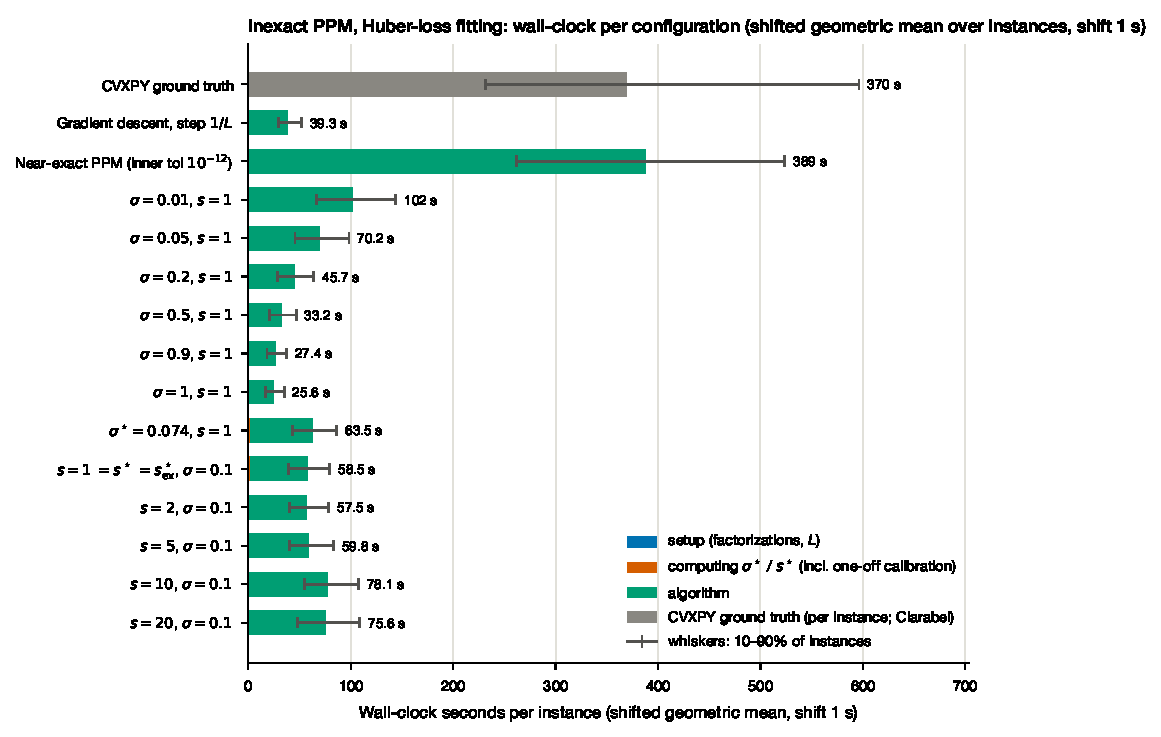
\includegraphics[width=\textwidth]{../results/numerical_experiments/ppm_huber/walltime_sgm.pdf}
    \caption{Wall-clock time per configuration on the Huber instances \Cref{eq:huber-loss-problem} with $n = 2000$ and $m = 3000$: the shifted geometric mean over the 100 instances of the setup time, of the time to compute $\sigma^\star$ or $s^\star$ where one is used (including a one-off calibration), and of the algorithm time, stacked.
    Whiskers span the 10th to the 90th percentile of the algorithm time, and the top bar is the CVXPY (Clarabel) solve time for scale.
    The configurations are gradient descent on \Cref{eq:huber-loss-problem}, the near-exact method, the $\sigma$ sweep at $s = 1$ (including $\sigma^\star$), and the $s$ sweep at $\sigma = 0.1$ (including $s^\star$).
    Sufficiently inexact runs are faster than both the near-exact method and gradient descent.}\label{fig:ppm-huber-wall-clock-times}
\end{figure}

\Cref{fig:ppm-huber-outer-convergence} compares the convergence behavior of the configurations; \Cref{fig:ppm-huber-outer-convergence-zoom} in \Cref{sec:additional-ppm} magnifies its outer-iteration panels.
Despite producing virtually identical suboptimality and stationarity residuals, the performance over the \emph{inner} work is different.
In fact, the near-exact PPM performs worse than all other configurations in this regard.
Moreover, the highly inexact choices of parameters, $\sigma=0.5$ and $\sigma=0.9$, outperform vanilla gradient descent in terms of the number of gradient evaluations.
Even $\sigma=0.2$ is competitive with gradient descent.

\begin{figure}
    \centering
    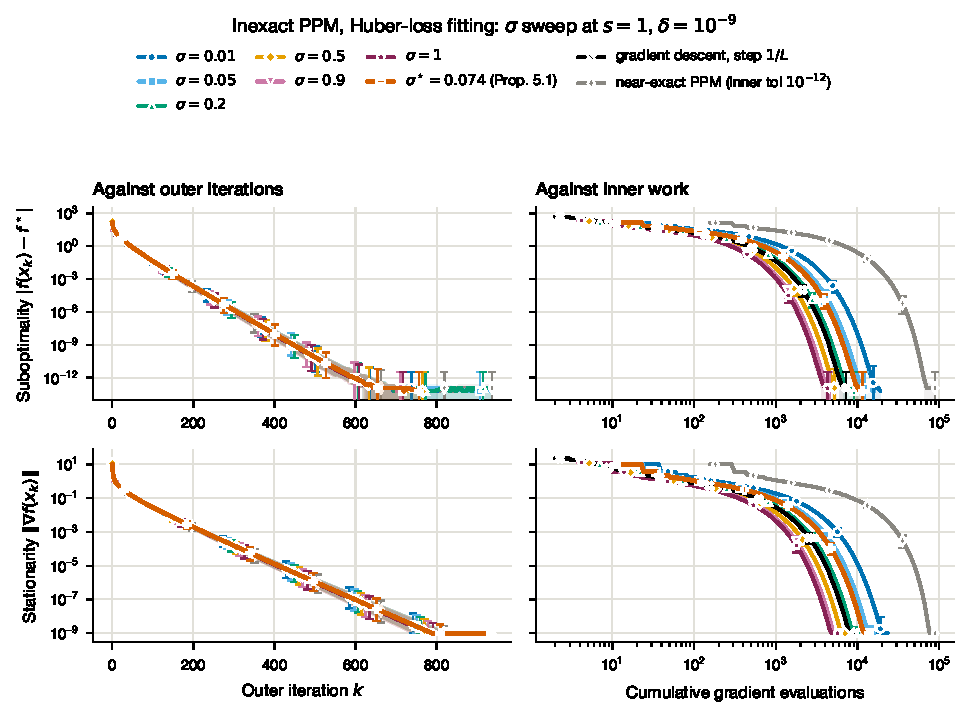
\includegraphics[width=\textwidth]{../results/numerical_experiments/ppm_huber/convergence_sigma.pdf}
    \caption{Convergence of \Cref{alg:stopping-time-algorithm} on the Huber instances \Cref{eq:huber-loss-problem} for the $\sigma$ sweep at $s = 1$, for $\sigma^\star$, and for the near-exact method: suboptimality $|f(x_k) - f^\star|$ (top) and stationarity $\norm{\nabla f(x_k)}$ (bottom) against outer iterations (left) and against cumulative gradient evaluations (right).
    Lines are medians over the 100 instances, bands interquartile ranges, and whiskers the 10th to the 90th percentiles; gradient descent has no outer iterations and appears against gradient evaluations only.
    The curves nearly coincide against outer iterations but separate widely against inner work, where the near-exact method is the slowest.}\label{fig:ppm-huber-outer-convergence}
\end{figure}

The magnified view in \Cref{fig:ppm-huber-outer-convergence-zoom} confirms that the convergence metrics are nearly indistinguishable, suggesting that there is little effect of inexactness on the outer iterations.
The theory predicts a multiplicative factor of $\frac{1+\sigma}{1-\sigma}$ in the worst-case convergence rate, which equals 19 for $\sigma = 0.9$.
This factor is not visible in the numerics, highlighting the pessimism of the theory.

The trajectory of the inexact iterates tends to closely follow that of the near-exact algorithm.
In \Cref{fig:ppm-huber-trajectories}, the near-exact solutions to the subproblems of the inexact PPM (hollow markers) closely match the trajectory of the near-exact PPM (dashed line).
The inexact method required 47 outer iterations ($K_\delta = 47$), but the near-exact method required only 22 ($K_\delta = 22$).
However, the inexact PPM with $\sigma = 0.9$ used only 142 gradient evaluations, whereas the near-exact PPM used 1,571 gradient evaluations, over 10 times the number of gradient evaluations.
\begin{figure}
    \centering
    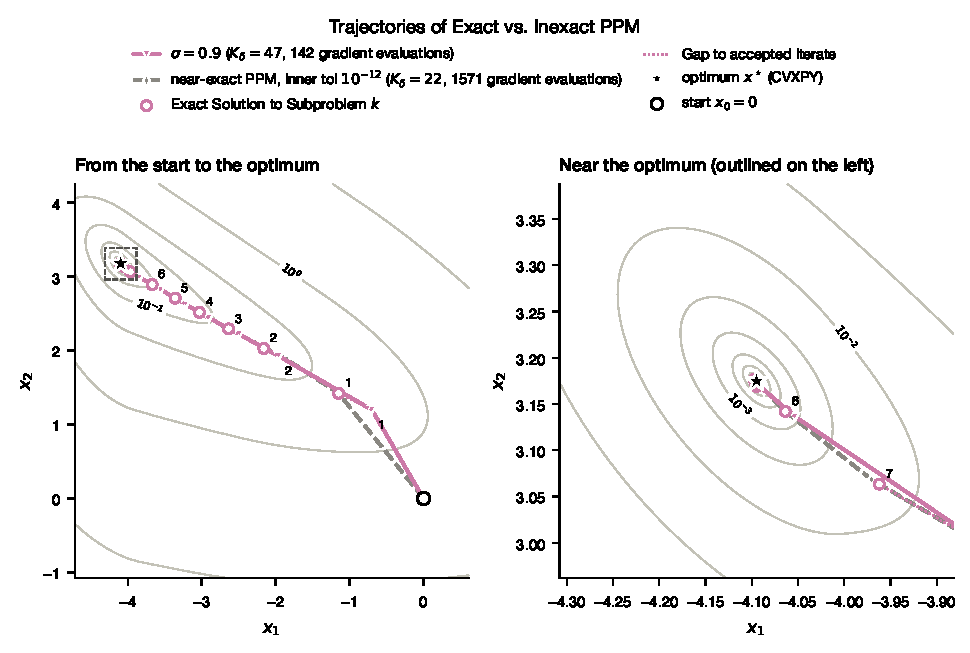
\includegraphics[width=\textwidth]{../results/numerical_experiments/ppm_huber_2d/trajectory_2d_exact.pdf}
    \caption{Accepted iterates of the near-exact method (dashed) and of one inexact run with $\sigma = 0.9$ and $s = 1$ on a two-dimensional Huber instance, over contours of $f - f^\star$: left, from the start $x_0 = 0$ to the optimum; right, the neighborhood of the optimum outlined on the left.
    Hollow markers are the exact solutions $J(w_k)$ of the subproblems that the inexact run approximated, joined to the accepted iterate by dotted segments; a point that passed several consecutive acceptance tests without an inner step carries all their iteration numbers.
    The inexact run takes 47 outer iterations against 22, but 142 gradient evaluations against 1,571.}\label{fig:ppm-huber-trajectories}
\end{figure}

Additionally, we compare the predicted cost of choosing different values of the stride $s$ (lines 4--10 of \Cref{alg:stopping-time-algorithm}).
The relaxed bound refers to that of \Cref{lem:check-frequency-s-star}, while the unrelaxed bound refers to \Cref{rem:b-star-remark}.
The unrelaxed bound gives a tighter bound, but only up to a nearly constant factor.
Moreover, the conservatism of \Cref{lem:check-frequency-s-star} can be seen in \Cref{fig:ppm-huber-optimal-b-star-model}, where increasing the stride does not seem to affect the time per outer iteration significantly.
The cost of checking depends on factors such as hardware types and availability, difficulty of subproblems, implementation details, and so forth, but using the $s^\star$ defined in \Cref{lem:check-frequency-s-star} seems to be a good heuristic.

\begin{figure}
    \centering
    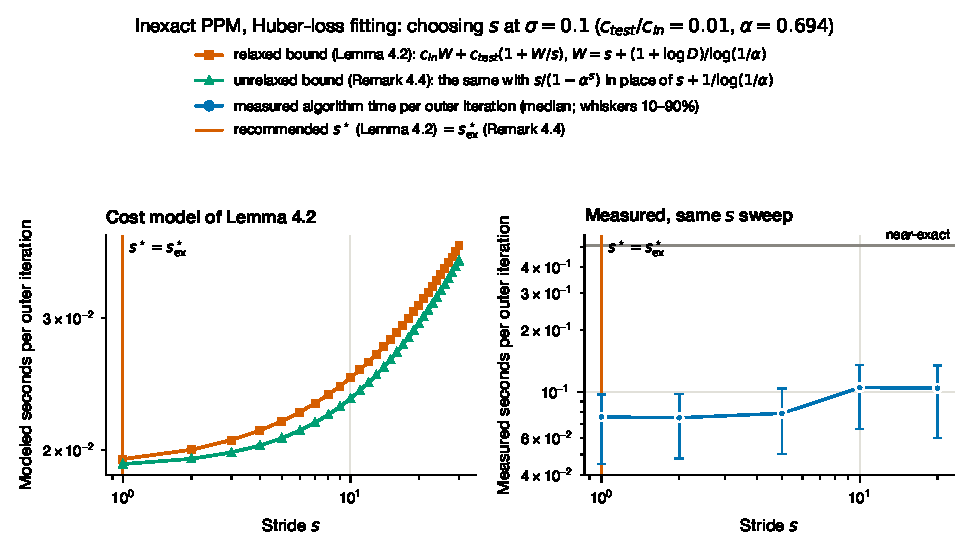
\includegraphics[width=\textwidth]{../results/numerical_experiments/ppm_huber/bstar_model.pdf}
    \caption{Choosing the stride on the Huber instances.
    Left, the modeled seconds per outer iteration as a function of $s$ from \Cref{lem:check-frequency-s-star} (relaxed bound) and from \Cref{rem:b-star-remark} (unrelaxed bound), with their integer minimizers marked; right, the measured seconds per outer iteration of the $s$ sweep at $\sigma = 0.1$ (median over the 100 instances; whiskers from the 10th to the 90th percentile), with the level of the near-exact method as a horizontal line.
    The relaxation shifts the model by a nearly constant factor, and the measured time is almost flat in $s$.}\label{fig:ppm-huber-optimal-b-star-model}
\end{figure}

\subsection{Inexact ADMM}\label{sec:numerical-experiments-admm}
In this section, we empirically study the performance of \Cref{alg:inexact-admm} on a quadratic program with linear equality constraints.
That is,
% \begin{align}
%     \min_{x\in\R^n} \quad & \frac{1}{2}x^\top Q x + d^\top x \label{eq:admm-qp}\\
%     \text{subject to} \quad &Ax = b, \notag
% \end{align}
\begin{equation}\label{eq:admm-qp}
    \begin{array}{ll}
    \text{minimize} & \frac{1}{2}x^\top Q x + d^\top x, \\
    \text{subject to} &Ax = b,
    \end{array}
\end{equation}
where $x\in\R^n$ is the optimization variable and $A\in\R^{m\times n}$, $Q\succ 0$, $d\in\R^n$, and $b\in\R^m$ are the problem data.
We take $m = 600$ and $n = 2000$ in these trials, with penalty $c = \frac{L}{10}$, where $L$ is the smoothness constant of the objective.
Our stopping tolerance is $\delta = 10^{-9}$.
The sweeps are the same as for the Huber instances: the $\sigma$ sweep runs at $s = 1$ and the stride sweep at $\sigma = 0.1$.
Every run starts from $z_0 = p_0 = 0$.
As before, we compare to the solution time of CVXPY using the Clarabel solver, but we also include a closed-form solution for the $x$-subproblem in \Cref{eq:admm-x-subproblem-numerical-experiments-qp}.
Since the optimality conditions for the $x$-subproblem \Cref{eq:admm-x-subproblem-numerical-experiments-qp} are a linear system, $(Q + cI)x = cz_k - d - p_k$, we compare an iterative solution to using a Cholesky factorization of the matrix $Q + cI$.
In large-scale applications, obtaining such a factorization may not be feasible, but this is still implemented in some well-known solvers such as OSQP \citep{osqp-original-paper}.

We sample $Q = V\diag(\lambda)V^\top$, where $\lambda$ is log-spaced in $[\kappa^{-1},1]$, $V$ is the orthogonal factor of the QR decomposition of a matrix with i.i.d.\ $\mathcal{N}(0,1)$ entries, and $\kappa = 10^4$.
This also shows that $\norm{Q}_2 = 1$ is the $L$-smoothness constant of the objective.
The regularized matrix $Q+cI$ appearing in the $x$-subproblem \Cref{eq:admm-x-subproblem-numerical-experiments-qp} has $\kappa_c := \kappa_2(Q + cI) = \frac{1+c}{10^{-4} +c} \leq 1 + \frac{L}{c}$.
We use the estimate $\kappa_c \leq 1 + \frac{L}{c} = 11$ for the estimation of parameters.
In this setup, the exact value is $\kappa_c \approx 10.99$, so this approximation is good for matrices with small eigenvalues.
The constraint matrix $A$ has i.i.d.\ $\mathcal{N}(0, n^{-1})$ entries.
We generate ground truth primal and dual solutions $x^\star\in\R^n$ and $\nu^\star\in\R^m$ with i.i.d.\ $\mathcal{N}(0, n^{-1})$ and $\mathcal{N}(0, m^{-1})$ entries, respectively.
The data $d$ and $b$ are computed such that the pair $(x^\star,\nu^\star)$ solves the Karush--Kuhn--Tucker (KKT) system, so that the ADMM dual $p_k$ converges to $-(Qx^\star + d) = A^\top\nu^\star$.
Since $Q\succ 0$ and $A$ is full rank, the solution is unique.
The subproblems \Cref{eq:admm-iterates} become
\begin{subequations}\label{eq:admm-iterates-numerical-experiments-qp}
\begin{align}
    x_{k} &\approx \argmin_{x} \left\{ \frac{1}{2}x^\top Q x + d^\top x + \ip{p_k}{x} + \frac{c}{2}\norm{x-z_k}^2 \right\}, \label{eq:admm-x-subproblem-numerical-experiments-qp}\\
    p_{k+1} &= p_k + c(x_{k}-z_k), \\
    z_{k+1} &= \argmin_{z}\left\{  \mathcal{I}_{\left\{ z \mid Az = b \right\}}(z) - \ip{p_{k+1}}{z} + \frac{c}{2}\norm{z-x_{k}}^2 \right\}. \label{eq:admm-z-subproblem-numerical-experiments-qp}
\end{align}
\end{subequations}
Substituting this into \Cref{alg:inexact-admm} yields the algorithm found in the code.
Note that the $z$-subproblem \Cref{eq:admm-z-subproblem-numerical-experiments-qp} is the projection of $x_k + p_{k+1}/c$ (of $x_k - a_k/c$ in \Cref{alg:inexact-admm}) onto the affine subspace $\{z \mid Az = b\}$, which can be done to machine precision.
The inexactness arises from the $x$-subproblem, which we internally solve using GMRES, since the optimality conditions are a positive definite linear system.
We remark that in this setup, $C_0 =4$ and $\sqrt{\alpha} = \frac{\sqrt{\kappa_c}-1}{\sqrt{\kappa_c}+1}$, so $\alpha\approx 0.288$.
The constants come from an application of the Chebyshev bound in the proof of \citet[Theorem 38.5]{Trefethen1997NumericalLinearAlgebra} to \citet[Proposition 4]{saad1986GMRES}.

The wall-clock times in \Cref{fig:admm-qp-wall-clock-times} demonstrate that the theory is fairly conservative.
Very inexact iterations appear to have \emph{better} performance than their exact counterparts.
We attribute this to the ability to move in generally the correct direction, even though the precise step may not be accurate.
However, all configurations using an iterative method to solve the $x$-subproblem in \Cref{eq:admm-x-subproblem-numerical-experiments-qp} are slower than using the Cholesky factorization of $Q + cI$.
We do not consider this to be a limitation, since in many applications such a closed-form solution is either not available or not feasible to implement.

\begin{figure}
    \centering
    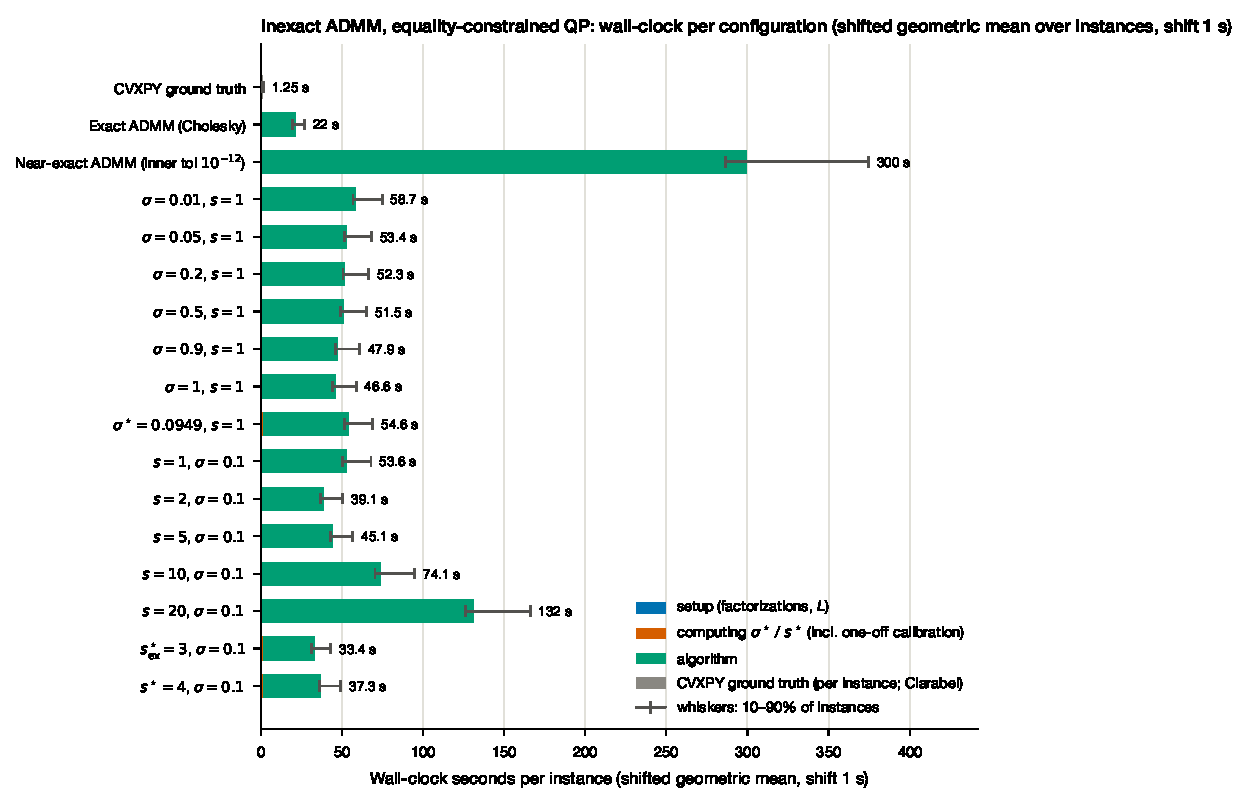
\includegraphics[width=\textwidth]{../results/numerical_experiments/admm_qp/walltime_sgm.pdf}
    \caption{Wall-clock time per configuration on the quadratic programs \Cref{eq:admm-qp} with $n = 2000$ and $m = 600$: the shifted geometric mean over the 100 instances of the setup time, of the time to compute $\sigma^\star$ or $s^\star$ where one is used (including a one-off calibration), and of the algorithm time, stacked.
    Whiskers span the 10th to the 90th percentile of the algorithm time, and the top bar is the CVXPY (Clarabel) solve time for scale.
    The configurations are exact ADMM with a Cholesky factorization of $Q + cI$, the near-exact method, the $\sigma$ sweep at $s = 1$ (including $\sigma^\star$), and the $s$ sweep at $\sigma = 0.1$ (including $s^\star$).
    Every configuration that uses GMRES is slower than the factorization, and the inexact ones are faster than the near-exact method.}\label{fig:admm-qp-wall-clock-times}
\end{figure}

The convergence behavior of the outer iterates in \Cref{fig:admm-qp-outer-convergence} is comparable across all configurations; \Cref{fig:admm-qp-outer-convergence-zoom} in \Cref{sec:additional-admm} magnifies its outer-iteration panels.
However, solving the subproblem to extremely high absolute accuracy (in this case, $10^{-12}$) is unnecessary and often detrimental.

\begin{figure}
    \centering
    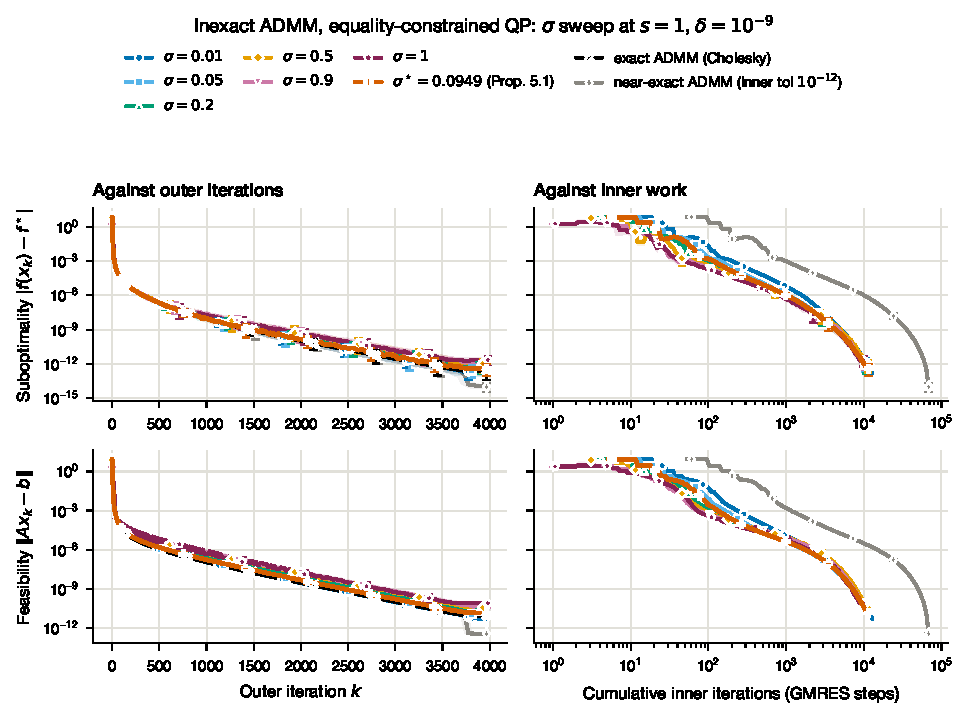
\includegraphics[width=\textwidth]{../results/numerical_experiments/admm_qp/convergence_sigma.pdf}
    \caption{Convergence of \Cref{alg:inexact-admm} on the quadratic programs \Cref{eq:admm-qp} for the $\sigma$ sweep at $s = 1$, for $\sigma^\star$, for the near-exact method, and for exact ADMM: suboptimality $|f(x_k) - f^\star|$ (top) and primal feasibility $\norm{Ax_k - b}$ (bottom) against outer iterations (left) and against cumulative GMRES iterations (right).
    Lines are medians over the 100 instances, bands interquartile ranges, and whiskers the 10th to the 90th percentiles; exact ADMM has no inner iterations and appears against outer iterations only.
    The outer-iteration curves are comparable across configurations, while the more inexact ones need the fewest GMRES iterations.}\label{fig:admm-qp-outer-convergence}
\end{figure}

The magnified view in \Cref{fig:admm-qp-outer-convergence-zoom} confirms that the convergence metrics are nearly indistinguishable, and in fact the more inexact configurations perform \emph{better} than the exact ones.
The inexact configurations outperform the theory, which is generally conservative.

As in the previous section, we compare the modeled cost of different choices of $s$ to the actual measured cost.
Numerically solving for a more precise $s^\star$ yields a better result, both theoretically and empirically, as seen in \Cref{fig:admm-qp-optimal-b-star-model}.
The setup costs of computing $s^\star$ or $\sigma^\star$ are included as the middle segment of each bar, but they are negligible compared to the overall cost of the algorithm and are not visible.
% However, this involves nonnegligible setup costs, as seen in the orange bars of \Cref{fig:admm-qp-wall-clock-times}.
\begin{figure}
    \centering
    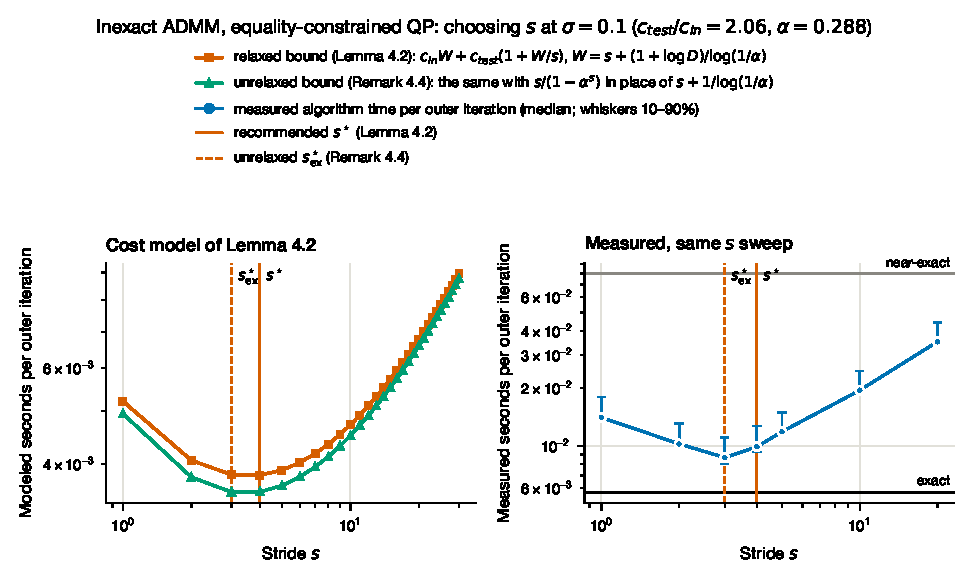
\includegraphics[width=\textwidth]{../results/numerical_experiments/admm_qp/bstar_model.pdf}
    \caption{Choosing the stride on the quadratic programs.
    Left, the modeled seconds per outer iteration as a function of $s$ from \Cref{lem:check-frequency-s-star} (relaxed bound) and from \Cref{rem:b-star-remark} (unrelaxed bound), with their integer minimizers marked; right, the measured seconds per outer iteration of the $s$ sweep at $\sigma = 0.1$ (median over the 100 instances; whiskers from the 10th to the 90th percentile), with the levels of exact ADMM and of the near-exact method as horizontal lines.
    The minimizer of the unrelaxed bound is the better choice, both in the model and in the measurement.}\label{fig:admm-qp-optimal-b-star-model}
\end{figure}

\subsection{Rotation Operator}
We first check the one-step decrease of \Cref{lem:one-step-decrease-inequality} on the two-dimensional Huber instance, and then on an operator for which the lemma is tight for exact steps.
On the two-dimensional Huber instance of \Cref{fig:ppm-huber-trajectories}, the decrease of $\norm{w_k - x^\star}^2$ at each accepted update is well above the amount that \Cref{lem:one-step-decrease-inequality} guarantees for every $\sigma$ (\Cref{fig:huber-fejer-ratio}).
The median over the accepted updates is between $1.77$ and $2.58$ times $\norm{\gamma z_k}^2$ for every $\sigma$ shown, including $\sigma^\star$, against a guarantee of $\frac{1-\sigma}{1+\sigma}$, so the factor $\frac{1+\sigma}{1-\sigma}$ of \Cref{thm:convergence-guarantee} is not reflected in the decrease per accepted step.
To show that this factor is not an artifact of the analysis, we repeat the experiment in two dimensions on the linear operator $\Bcal(x) = U(x-x^\star)$, where $U=\begin{bmatrix}
    0 & -1 \\ 1 & 0
\end{bmatrix}$ is the rotation by a quarter turn.
The operator $\Bcal$ is monotone (but not a gradient).
The instance has $x^\star$ at distance $5$ from the start $x_0 = 0$, and the runs use the same $\sigma$ sweep as before at $s = 1$, with $\delta = 10^{-9}$ and an inner residual of $10^{-12}$ for the near-exact method.
The exact proximal step $w^+$ satisfies $\norm{w - x^\star}^2 - \norm{w^+ - x^\star}^2 = \norm{w - w^+}^2$\footnote{The critical property here is skew-symmetry of the operator.
One could take any higher-dimensional skew-symmetric affine operator to get the same exact decrease equality.} and \Cref{lem:one-step-decrease-inequality} is tight for exact steps.
The inner solver is Richardson iteration on the resolvent residual with the step that minimizes its contraction factor, which satisfies \Cref{assumption:inner-work-contraction} with $C_0 = 1$ and $\alpha = \frac{\gamma^2}{1+\gamma^2} = 0.8$ for $\gamma = 2$.
\Cref{fig:torsion-trajectories} shows the paths and \Cref{fig:torsion-fejer-ratio} the observed decrease against its guarantee; the convergence of the sweep, in the layout of \Cref{fig:ppm-huber-outer-convergence}, is \Cref{fig:torsion-convergence} in \Cref{sec:additional-rotation}.
The near-exact method needs $K_\delta = 26$ outer iterations, $\sigma = 0.5$ needs $62$, $\sigma = 0.9$ needs $48$, and $\sigma = 1$ needs $235$, and the median decrease per $\norm{\gamma z_k}^2$ is $1.00$ for the near-exact method, $1.02$ at $\sigma = 0.01$, $0.41$ at $\sigma = 0.5$, $0.28$ at $\sigma = 0.9$, and $0.047$ at $\sigma = 1$, against guarantees of $1$, $0.98$, $0.33$, $0.053$, and $0$.
\begin{figure}
    \centering
    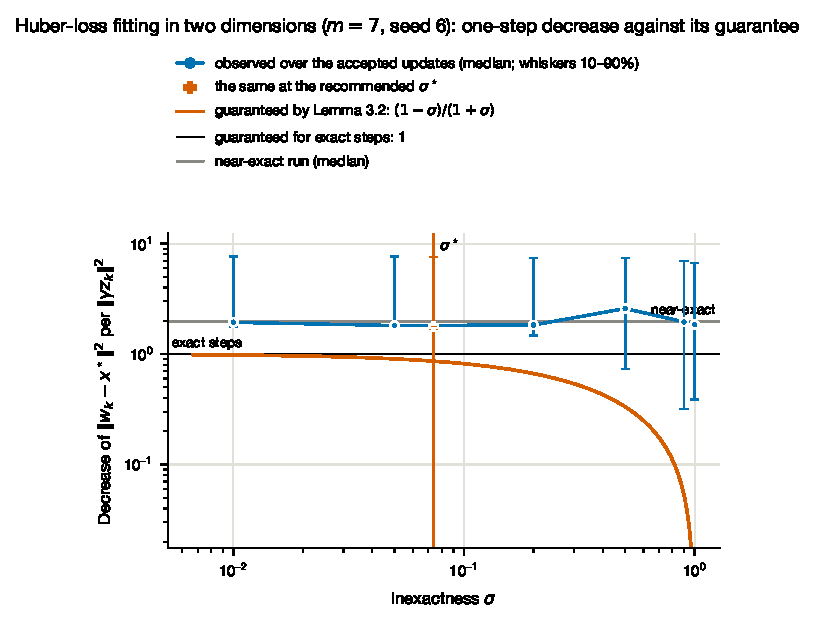
\includegraphics[width=0.7\textwidth]{../results/numerical_experiments/ppm_huber_2d/fejer_ratio.pdf}
    \caption{The decrease of $\norm{w_k - x^\star}^2$ at each accepted update divided by $\norm{\gamma z_k}^2$ on the two-dimensional Huber instance of \Cref{fig:ppm-huber-trajectories}, for the $\sigma$ sweep at $s = 1$ and for $\sigma^\star$ (median over the accepted updates; whiskers from the 10th to the 90th percentile), against the guarantee $\frac{1-\sigma}{1+\sigma}$ of \Cref{lem:one-step-decrease-inequality}, the level $1$ guaranteed for exact steps, and the level observed for the near-exact method.
    The observed decrease stays near the level of exact steps for every $\sigma$.}\label{fig:huber-fejer-ratio}
\end{figure}
\begin{figure}
    \centering
    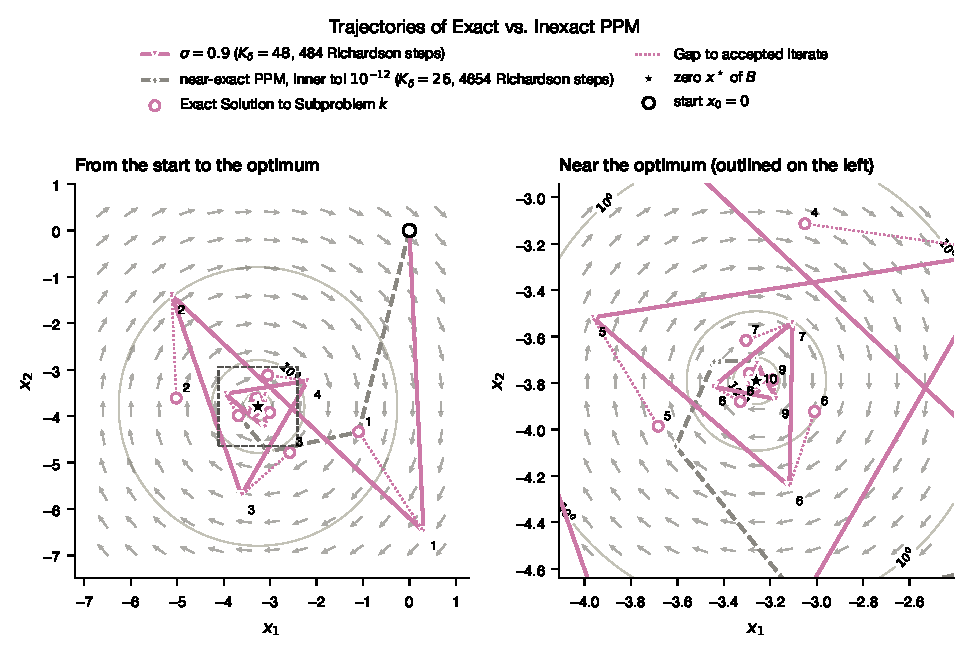
\includegraphics[width=\textwidth]{../results/numerical_experiments/torsion_operator/trajectory_2d_exact.pdf}
    \caption{Accepted iterates of \Cref{alg:stopping-time-algorithm} on the rotation operator $\Bcal(x) = U(x-x^\star)$ for $\sigma = 0.9$ (solid) and for the near-exact method (dashed), at $s = 1$, over contours of $\norm{x - x^\star}$; arrows give the direction of $-\Bcal$, and the right panel magnifies the neighborhood of $x^\star$ outlined on the left.
    Since $\Bcal$ is skew-symmetric, each exact step decreases $\norm{w - x^\star}^2$ by exactly $\norm{w - w^+}^2$, while the inexact iterates wander around $x^\star$ and take 48 outer iterations against 26.}\label{fig:torsion-trajectories}
\end{figure}
\begin{figure}
    \centering
    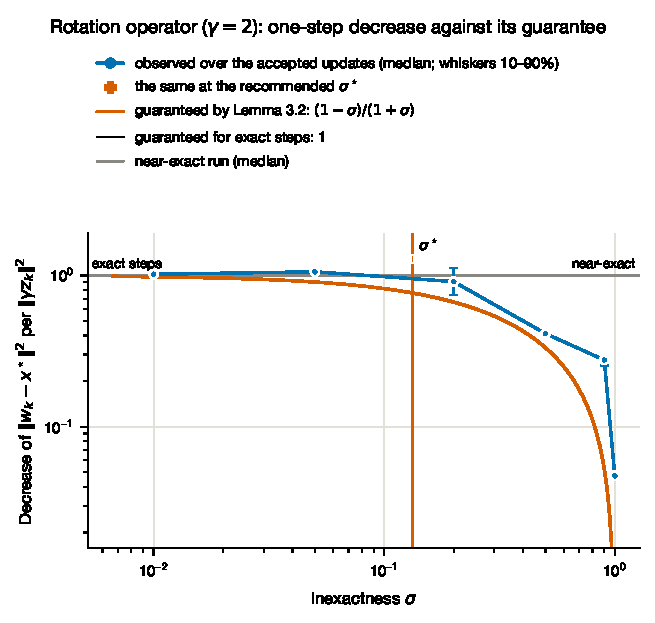
\includegraphics[width=0.7\textwidth]{../results/numerical_experiments/torsion_operator/fejer_ratio.pdf}
    \caption{The decrease of $\norm{w_k - x^\star}^2$ at each accepted update divided by $\norm{\gamma z_k}^2$ on the rotation operator of \Cref{fig:torsion-trajectories}, for the $\sigma$ sweep at $s = 1$ and for $\sigma^\star$ (median over the accepted updates; whiskers from the 10th to the 90th percentile), against the guarantee $\frac{1-\sigma}{1+\sigma}$ of \Cref{lem:one-step-decrease-inequality}, the level $1$ guaranteed for exact steps, and the level observed for the near-exact method.
    The near-exact run attains the exact level, and the inexact runs stay above their guarantee but drop well below the exact level for $\sigma \geq 0.5$.}\label{fig:torsion-fejer-ratio}
\end{figure}

\section{Conclusion}
We analyzed the expected inner work of proximal point methods for solving a monotone inclusion problem in a Hilbert space.
Equipped with a contractive inner procedure for computing the resolvent, we provide a quantitative bound on the amount of expected inner work required to solve the monotone inclusion problem to a given accuracy.
Our framework encompasses a broad variety of popular operator splitting algorithms, and we provide principled heuristics for selecting algorithm parameters a priori.
Numerical experiments validate our findings and suggest that in practice, many algorithms can tolerate significant amounts of inexactness.

Many questions remain open.
The $\Expect[K_\delta]$ term in \Cref{thm:total-inner-work-bound} opens the door to considering average-case complexity, rather than the worst-case performance.
Moreover, the choice of problem parameters is not only problem-sensitive, but also sensitive to the choice of inner procedure used.
Providing more thorough guidelines on the selection of parameters would be useful in practice.
Also of interest is differentiating which inner solvers are more compatible with certain outer solvers, and providing guidance on when to use a particular splitting or method over another.
Another promising direction is an adaptive choice of parameters.
The analysis of this work assumes that algorithm parameters are fixed, but in practice this is undesirable.
Incorporating an analysis of adaptive parameter selection would bring the theory closer to practice.
Another direction would be to relax the requirement in \Cref{alg:stopping-time-algorithm} that $\Ccal z_k \in\Acal u_k$, for cases where finding a member of $\Acal u_k$ is difficult, such as the case where the proximal step is projection onto a convex set.


\appendix
\section{Tightness of Bounds}\label{sec:tightness-of-bounds}
Here, we consider the tightness of the bounds of \Cref{sec:inner-work-guarantees}.

\subsection{Tightness of \texorpdfstring{$G_{\sigma}$}{G\_sigma} and \texorpdfstring{$H_{\sigma}$}{H\_sigma}}
\begin{remark}\label{rem:warm-start-sharp}
    The constant $G_\sigma$ in \Cref{eq:warm-start-bound} is sharp.
    Fix $\sigma$ and $r>0$, let $\varepsilon\in[\sigma r,\frac{\sigma r}{1-\sigma}]$ maximize $\Phi$ in \Cref{eq:warm-start-quadratic}, and set, for an orthonormal pair $(v_1,v_2)$,
    \begin{align}
        e_J &= \norm{e_J} v_1, \\ 
        e_R &= \norm{e_R} v_2, \\
        \gamma\bar z &= \frac{r}{\varepsilon}(-\norm{e_J} v_1 + \norm{e_R} v_2),
    \end{align}
    which is possible because $\norm{e_J}^2\geq0$ for $\varepsilon\geq\sigma r$ and $\norm{e_R}^2\geq0$ for $\varepsilon\leq\frac{\sigma r}{1-\sigma}$.
    This definition is not circular since we have
    \begin{align}
        \norm{e_J}^2 &= \frac{\varepsilon(\varepsilon^2 - \sigma^2r^2)}{\sigma^2(\varepsilon + 2r)}, \\
        \norm{e_R}^2 &= \varepsilon^2 - \norm{e_J}^2.
    \end{align}
    Moreover, $\norm{\gamma\bar z} = r$, $\ip{e_J}{e_R} = 0$, $\norm{e_J+e_R} = \varepsilon = \sigma\norm{e_J - \gamma\bar z}$, and $\ip{\gamma\bar z}{e_R-e_J} = r\norm{e_R-e_J}$, so every inequality in the proof holds with equality and $\norm{\gamma\bar z + e_J + 2e_R}^2 = \Phi(\varepsilon) = G_\sigma^2r^2$.
    Such a configuration is realized by an accepted pair: for any $\bar y$, the two-point set $\{(\bar y, \bar z), (\bar y + e_J, \bar z + e_R/\gamma)\}$ is monotone and therefore extends to a maximal monotone operator $\Bcal$ \citep[Theorem 20.21]{bauschkeConvexAnalysisMonotone2017}, for which $\bar y = J(w)$ and $\gamma\bar z = R(w)$ at $w = \bar y + \gamma\bar z$, and $(y,z) = (\bar y + e_J, \bar z + e_R/\gamma)$ is a graph pair at $w$ with residual $e = e_J + e_R$ that passes the relative test with equality.
    For $\sigma\leq\sigma_1$ the extremal configuration is $e_J = 0$, $e_R = \sigma R(w)$: the inner solver returns the exact resolvent point $y = J(w)$, but with $\gamma z = (1+\sigma)R(w)$.
    For $\sigma\geq\sigma_2$ it is $e_R = 0$, $e_J = -\frac{\sigma}{1-\sigma}R(w)$.

    The constant $H_\sigma$ in \Cref{eq:residual-drift-bound} is sharp as well, and here we can construct an explicit operator.
    Let $\Hcal = \Dcal = \R^2$, $\Ccal = I$, and $\Acal = \Bcal = \partial f$ with $f(y) = \frac{r}{\gamma}\left(|y_1| + \sigma H_\sigma|y_2|\right)$, a weighted $\ell_1$ norm, so that $J$ is the soft-thresholding map $J(w) = \left(\sign(w_1)\max\{|w_1| - r, 0\},\, \sign(w_2)\max\{|w_2| - \sigma H_\sigma r, 0\}\right)$.
    Fix $w_k = (w_1, 0)$ with $w_1\geq\frac{2r}{1-\sigma^2}$, so that $J(w_k) = (w_1 - r, 0)$ and $R(w_k) = (r, 0)$, and let the accepted pair be
    \begin{align}
        y_k = J(w_k) - \frac{\sigma^2}{1-\sigma^2}R(w_k) = \left(w_1 - \frac{r}{1-\sigma^2},\, 0\right), \qquad \gamma z_k = (r, \sigma H_\sigma r),
    \end{align}
    a graph pair because $\gamma\Bcal(y_k) = \{r\}\times[-\sigma H_\sigma r, \sigma H_\sigma r]$ (as $y_{k,1}>0$ and $y_{k,2} = 0$).
    In the notation of the proof, $e_J = -\frac{\sigma^2}{1-\sigma^2}R(w_k)$ and $e_R = (0, \sigma H_\sigma r)\perp e_J$, so $\norm{e_R} = \frac{\sigma r}{\sqrt{1-\sigma^2}}$ attains the bound on $\norm{e_R}$, and the residual $e_k = e_J + e_R$ satisfies $\norm{e_k}^2 = \frac{\sigma^4r^2}{(1-\sigma^2)^2} + \frac{\sigma^2r^2}{1-\sigma^2} = \frac{\sigma^2r^2}{(1-\sigma^2)^2} = \sigma^2\norm{y_k - w_k}^2$: the relative test passes with equality (and the terminal test fails whenever $\gamma\delta<\norm{\gamma z_k} = \frac{r}{\sqrt{1-\sigma^2}}$).
    Then $w_{k+1} = w_k - \gamma z_k = (w_1 - r, -\sigma H_\sigma r)$ with $w_1 - r>r$, so $J(w_{k+1}) = (w_1 - 2r, 0)$, $R(w_{k+1}) = (r, -\sigma H_\sigma r) = R(w_k) - e_R$, and
    \begin{align}
        \norm{R(w_{k+1})}^2 = r^2 + \sigma^2H_\sigma^2r^2 = \norm{R(w_k)}^2 + \norm{e_R}^2 = \frac{r^2}{1-\sigma^2} = H_\sigma^2\norm{R(w_k)}^2,
    \end{align}
    so both inequalities leading to \Cref{eq:drift-quadrature} hold with equality.
    The extremal configurations for the two constants differ: for $G_\sigma$ (with $\sigma\leq\sigma_1$) the error $e_R$ in $\gamma z_k$ is aligned with $R(w_k)$, whereas for $H_\sigma$ it is orthogonal to $R(w_k)$ and as large as the relative test allows, since \Cref{eq:drift-quadrature} adds it in quadrature.
    The first coordinate of this example is the instance of \Cref{rem:inner-work-sharpness}.
\end{remark}


\begin{remark}[Sharpness of \Cref{thm:stopping-time-concentration,thm:total-inner-work-bound,thm:deterministic-inner-work}]\label{rem:inner-work-sharpness}
    The per-step bound \Cref{eq:deterministic-per-step} is attained, for every $\sigma\in(0,1)$, $s$, $\alpha$, and $C_0$, by the following instance.
    Let $\Hcal = \Dcal = \R$, $\Ccal = I$, $\gamma = 1$, and $\Acal = \Bcal = \partial(r|\cdot|)$ with $r>\delta$, so that $J(w) = w - r$ and $R(w) = r$ for $w>r$, and let $w_0>r$.
    At an outer iteration with $w_k>r$, so that $\norm{R(w_k)} = r$, let the inner procedure return
    \begin{align}
        y^l &= J(w_k) + t_l R(w_k), \\
        z^l &= R(w_k)/\gamma, \\
        t_l &:= \sqrt{C_0}\,\alpha^{l/2}t_0 \quad(l \geq 1), \\
        t_0 &:= \frac{\norm{\gamma z^0 + y^0 - w_k}}{r},
    \end{align}
    that is, $y^l$ moves along the segment from $J(w_k)$ toward $w_k$ while the operator value stays exact.
    Then $y^l>0$, so $(y^l,z^l)\in\gra\Bcal$, and the residual is $e^l = t_l R(w_k)$.
    Thus, $\norm{e^l}^2 = C_0\alpha^l\norm{e^0}^2$ for $l \geq 1$.
    The relative test $\norm{e^l}\leq\sigma\norm{y^l - w_k} = \sigma|1-t_l|r$ holds if and only if $t_l\leq\frac{\sigma}{1+\sigma}$; i.e., if and only if $\norm{e^l}\leq\frac{\sigma}{1+\sigma}\norm{R(w_k)}$; and the terminal test fails because $\norm{z^l} = r>\delta$.
    Hence the inner loop exits at the first check at which the sufficient condition used in the proof of \Cref{thm:stopping-time-concentration} holds, and $N_k = s\lceil\logp\tilde\beta_k/(s\log(1/\alpha))\rceil$ exactly (whenever $\norm{e^0}>\frac{\sigma}{1+\sigma}\norm{R(w_k)}$, which is the case for $k\geq1$ below).
    Since $z$ is exact, the outer step is the exact proximal step $w_{k+1} = J(w_k)$, and the next warm start is $e^0_{k+1} = e_k + \gamma z_k = (1+t_{\mathrm{exit}})R(w_k)$ with $t_{\mathrm{exit}}\leq\frac{\sigma}{1+\sigma}$, so that $\norm{e^0_{k+1}}\leq\frac{1+2\sigma}{1+\sigma}\norm{R(w_k)}$ and, for $k\geq1$,
    \begin{align}
        \tilde\beta_k\leq\frac{(1+2\sigma)^2C_0}{\sigma^2}\,\frac{\norm{R(w_{k-1})}^2}{\norm{R(w_k)}^2} = \frac{D}{(1+\sigma)^2}\,\frac{\norm{R(w_{k-1})}^2}{\norm{R(w_k)}^2}\qquad(\sigma\leq\sigma_1),
    \end{align}
    with equality in the inequality when $t_{\mathrm{exit}} = \frac{\sigma}{1+\sigma}$, which is approached for $s = 1$ as $\alpha\to1$.
    A randomized variant of the same instance, in which the residual decreases deterministically to just above the threshold $\frac{\sigma}{1+\sigma}\norm{R(w_k)}$ and then, at each inner iteration, is either solved exactly with probability $1-\alpha$ or left unchanged, makes Markov's inequality in the proof of \Cref{thm:stopping-time-concentration} tight at every check.
    It shows that the bound on $\Expect_k[N_k]$ there, and with it the per-iteration constant $\frac{s}{1-\alpha^s}$ of \Cref{thm:total-inner-work-bound}, can be approached arbitrarily closely.

    The total bounds \Cref{eq:total-inner-work-bound,eq:deterministic-total} are, however, never attained when $K_\delta \geq 1$.
    The constant $D = \frac{(1+\sigma)^2C_0G_\sigma^2}{\sigma^2}$ combines the threshold factor $\frac{1+\sigma}{\sigma}$ of \Cref{thm:stopping-time-concentration}, which is used fully only when an inner loop exits at the forced level, with an accepted residual $\norm{e_k}\leq\frac{\sigma}{1+\sigma}\norm{R(w_k)}$, with the warm-start factor $G_\sigma$ of \Cref{lem:warm-start-bounds}, which by \Cref{rem:warm-start-sharp} requires an accepted residual $\norm{e_k}\geq\sigma\norm{R(w_k)}$ at the same iteration.
    The two cannot hold simultaneously.
    Quantitatively, $\norm{e^0_{k+1}}\leq\norm{R(w_k)} + 2\norm{e_k}$ always, so a forced exit yields $\norm{e^0_{k+1}}\leq\frac{1+3\sigma}{1+\sigma}\norm{R(w_k)}<G_\sigma\norm{R(w_k)}$.
    In the instance above the exit is at the forced level and the warm start is $G_\sigma\norm{R(w_k)}/(1+\sigma)$.
    Exiting instead at $\norm{e_k} = \sigma\norm{R(w_k)}$ with the extremal pair of \Cref{rem:warm-start-sharp} gives the same per-iteration cost, namely $\frac{(1+2\sigma)^2C_0}{\sigma^2}$ in place of $D$ in both cases.
    Consequently, for $\sigma\leq\sigma_1$, no constant smaller than $\frac{D}{(1+\sigma)^2} = \frac{(1+2\sigma)^2C_0}{\sigma^2}$ can replace $D$ in \Cref{eq:total-inner-work-bound,eq:deterministic-total} (take the instance above with $s = 1$ and $\alpha\to1$).
    While $D$ itself is never attained, $D$ is sharp up to the factor $(1+\sigma)^2$, i.e., up to $\frac{2\log(1+\sigma)}{\log(1/\alpha)}\leq\frac{2\sigma}{\log(1/\alpha)}$ inner iterations per outer iteration, and the ceiling in \Cref{eq:deterministic-per-step} accounts for fewer than $s$ further inner iterations per outer iteration.
    % For the values of $\sigma^\star$ of \Cref{prop:optimal-sigma-gradient-descent-inside-ppm}, this is a few percent of the per-iteration work $\frac{\log D}{\log(1/\alpha)}\approx\frac{2\log(1/\sigma)}{\log(1/\alpha)}$.
\end{remark}

\section{Additional Numerical Results}\label{sec:additional-numerics}
This appendix collects figures that supplement \Cref{sec:numerical-experiments} without being needed to follow it: magnified views of the convergence figures and the convergence of the rotation-operator sweep.
Its subsections mirror those of \Cref{sec:numerical-experiments}, so that further details of each study can be added in place.

\subsection{Inexact Proximal Point}\label{sec:additional-ppm}
\Cref{fig:ppm-huber-outer-convergence-zoom} magnifies the outer-iteration panels of \Cref{fig:ppm-huber-outer-convergence} on the early iterations and on the final approach, where the curves of the $\sigma$ sweep coincide at full scale.
\begin{figure}
    \centering
    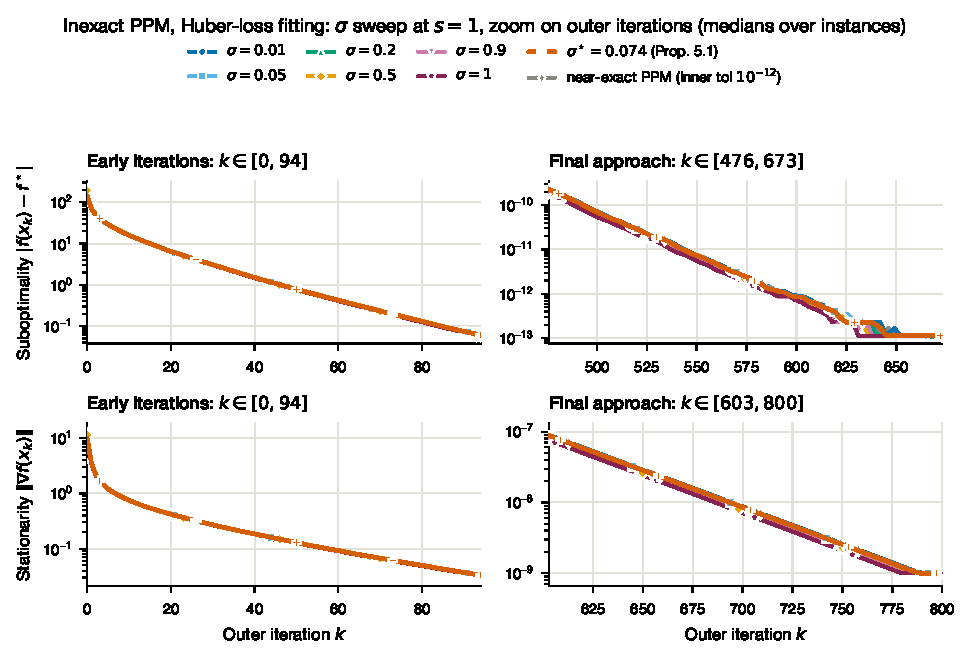
\includegraphics[width=\textwidth]{../results/numerical_experiments/ppm_huber/convergence_sigma_zoom.pdf}
    \caption{The outer-iteration panels of \Cref{fig:ppm-huber-outer-convergence} on two windows: the first 12\% of the median run (left) and the final approach of each metric to its plateau (right), as medians over the 100 instances only, so that curves that coincide at full scale can be told apart.}\label{fig:ppm-huber-outer-convergence-zoom}
\end{figure}
\FloatBarrier

\subsection{Inexact ADMM}\label{sec:additional-admm}
\Cref{fig:admm-qp-outer-convergence-zoom} does the same for \Cref{fig:admm-qp-outer-convergence}.
\begin{figure}
    \centering
    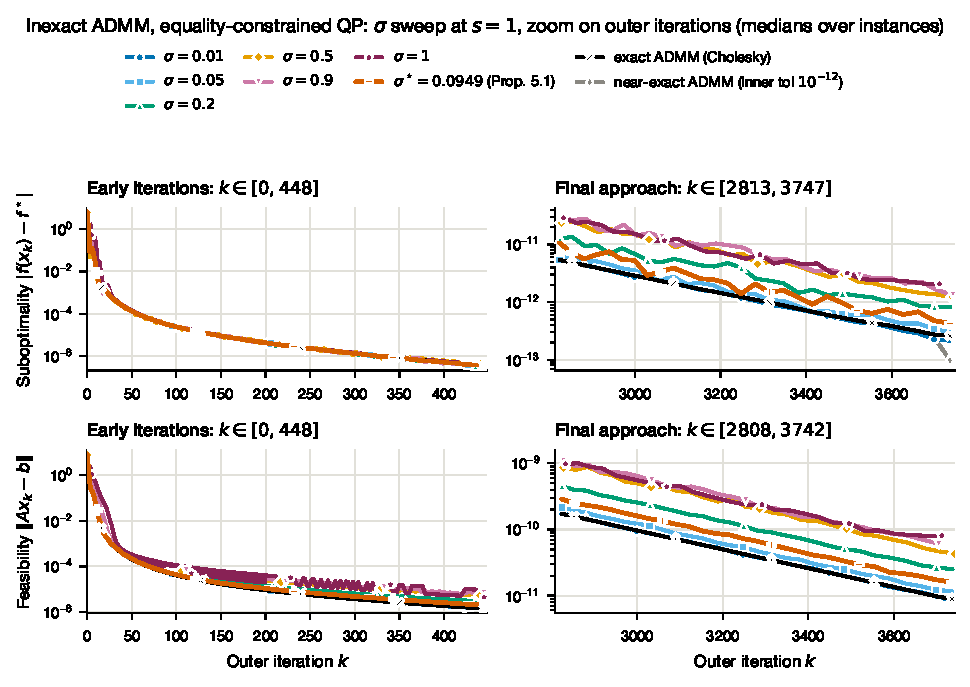
\includegraphics[width=\textwidth]{../results/numerical_experiments/admm_qp/convergence_sigma_zoom.pdf}
    \caption{The outer-iteration panels of \Cref{fig:admm-qp-outer-convergence} on two windows: the first 12\% of the median run (left) and the final approach of each metric to its plateau (right), as medians over the 100 instances only, so that curves that coincide at full scale can be told apart.}\label{fig:admm-qp-outer-convergence-zoom}
\end{figure}
\FloatBarrier

\subsection{Rotation Operator}\label{sec:additional-rotation}
\Cref{fig:torsion-convergence} shows the convergence of the $\sigma$ sweep on the rotation operator of \Cref{fig:torsion-trajectories} in the layout of the main studies.
\begin{figure}
    \centering
    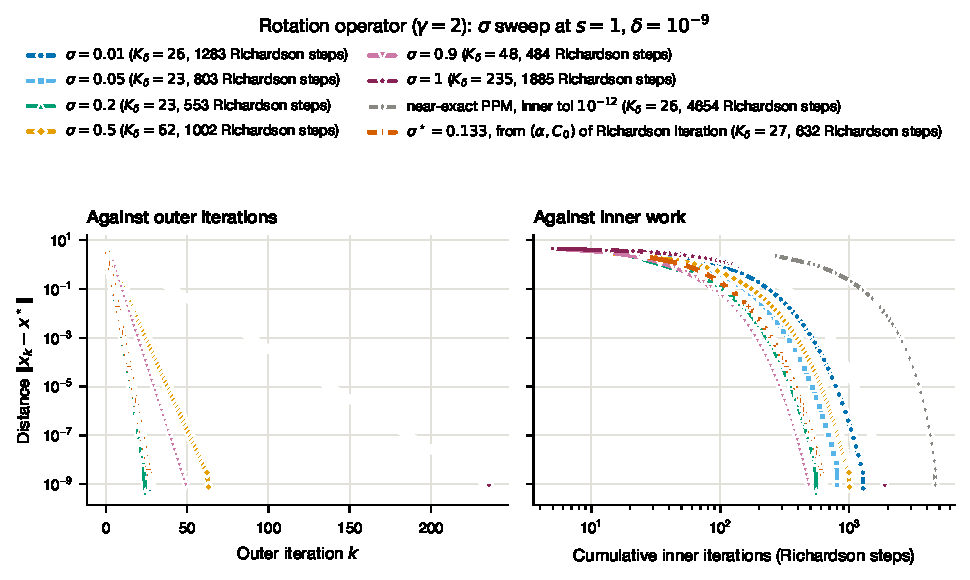
\includegraphics[width=\textwidth]{../results/numerical_experiments/torsion_operator/convergence_sigma.pdf}
    \caption{Convergence on the rotation operator of \Cref{fig:torsion-trajectories} for the $\sigma$ sweep at $s = 1$, for $\sigma^\star$, and for the near-exact method, in the layout of \Cref{fig:ppm-huber-outer-convergence}: the distance $\norm{x_k - x^\star} = \norm{\Bcal(x_k)}$ against outer iterations (left) and against cumulative Richardson steps (right).
    There is a single instance, so each curve is one run and there are no bands.
    The near-exact method stops after 26 outer iterations and the $\sigma = 1$ run after 235.}\label{fig:torsion-convergence}
\end{figure}

\printbibliography


\end{document}